%%%%%%%%%%%%%%%%%%%%%%%%%%%%%%%%%%%%%%%%%%%%%%%%%%%%%%%%%%%%%%%%%%%%%%%%%%%%%%%%
% Preámbulo                                                                    %
%%%%%%%%%%%%%%%%%%%%%%%%%%%%%%%%%%%%%%%%%%%%%%%%%%%%%%%%%%%%%%%%%%%%%%%%%%%%%%%%

\documentclass[11pt,a4paper,titlepage,twoside,openright,openbib]{report}

%%% RELACIÓN DE VARIABLES A PERSONALIZAR %%%
%\def\lingua{gal}
\def\lingua{esp} % descomenta esta liña se redactarás a memoria en español
%\def\lingua{eng} % descomenta esta liña se redactarás a memoria en inglés
\def\nome{Adrián Insua Yañez}                             % substitúe aquí o teu nome
\def\nomedirectorA{Carlos Gómez Rodríguez}             % substitúe aquí o nome de quen dirixe
\def\nomedirectorB{Sonia González Vázquez}
\def\titulo{Sistema Deep Learning para el análisis de sentimientos en opiniones de productos para la ordenación de resultados de un buscador semántico} % substitúe aquí o título do teu TFG
\def\mencion{COMPUTACIÓN}                        % descomenta a mención correspondente
%\def\mencion{COMPUTACIÓN}
%\def\mencion{ENXEÑARÍA DO SOFTWARE}
%\def\mencion{ENXEÑARÍA DE COMPUTADORES}
%\def\mencion{SISTEMAS DE INFORMACIÓN}
%\def\mencion{TECNOLOXÍAS DA INFORMACIÓN}

%\def\renomearcadros{si} % descomenta esta liña se redactas a memoria en español e prefires que
                         % os "cuadros" e o "índice de cuadros" se renomeen
                         % a "tablas" e "índice de tablas" respectivamente

\usepackage{estilo_tfg}
\usepackage{endnotes}

\newcommand{\SubItem}[1]{
	{\setlength\itemindent{15pt} \item[-] #1}
}

% Lista de paquetes potencialmente interesantes (uso baixo demanda)

% \usepackage{alltt}       % proporciona o entorno alltt, semellante a verbatim pero que respecta comandos
% \usepackage{enumitem}    % permite personalizar os entornos de lista
% \usepackage{eurofont}    % proporciona o comando \euro
\usepackage{float}       % permite máis opcións para controlar obxectos flotantes (táboas, figuras)
% \usepackage{hhline}      % permie personalizar as liñas horizontais en arrays e táboas
% \usepackage{longtable}   % permite construir táboas que ocupan máis dunha páxina
% \usepackage{lscape}      % permite colocar partes do documento en orientación apaisada
% \usepackage{moreverb}    % permite personalizar o entorno verbatim
% \usepackage{multirow}    % permite crear celdas que ocupan varias filas da mesma táboa
% \usepackage{pdfpages}    % permite insertar ficheiros en PDF no documento
% \usepackage{rotating}    % permite diferentes tipos de rotacións para figuras e táboas
% \usepackage{subcaption}  % permite a inclusión de varias subfiguras nunha figura
% \usepackage{tabu}        % permite táboas flexibles
% \usepackage{tabularx}    % permite táboas con columnas de anchura determinada

%%%%%%%%%%%%%%%%%%%%%%%%%%%%%%%%%%%%%%%%%%%%%%%%%%%%%%%%%%%%%%%%%%%%%%%%%%%%%%%%
% Corpo                                                                        %
%%%%%%%%%%%%%%%%%%%%%%%%%%%%%%%%%%%%%%%%%%%%%%%%%%%%%%%%%%%%%%%%%%%%%%%%%%%%%%%%

\begin{document}

 %%%%%%%%%%%%%%%%%%%%%%%%%%%%%%%%%%%%%%%%
 % Preliminares do documento            %
 %%%%%%%%%%%%%%%%%%%%%%%%%%%%%%%%%%%%%%%%

 \begin{titlepage}
  
  \hspace*{128pt}
  \textcolor{udcpink}{{\fontencoding{T1}\fontfamily{phv}\selectfont Facultade de Informática}}\\[-32pt]

  \begin{center}
    
\includegraphics[scale=0.3]{imaxes/udc}\\[35pt]

    {\large TRABALLO FIN DE GRAO \\
            GRAO EN ENXEÑARÍA INFORMÁTICA \\
            MENCIÓN EN \mencion } \\[100pt]
    
    \begin{huge}
      \begin{spacing}{1.3}
        \bfseries \titulo
      \end{spacing}
    \end{huge}
  \end{center}
  
  \vfill
  
  \begin{flushright}
    {\large
    \begin{tabular}{ll}
      {\bf Estudante:} & \nome \\
      {\bf Dirección:} & \nomedirectorA \\ % COPIA E PEGA ESTA LIÑA MÁIS VECES SE O PRECISAS
      {\bf Dirección:} & \nomedirectorB \\ % COPIA E PEGA ESTA LIÑA MÁIS VECES SE O PRECISAS
    \end{tabular}}
  \end{flushright}
  \rightline{A Coruña, \datasimple\today.}
\end{titlepage}

 \paxinaenbranco
 \dedicatoria{ A mi familia y amigos por su apoyo incondicional} % escribe neste comando o teu texto de dedicatoria
l
 \paxinaenbranco
 \paxinaenbranco
 \begin{agradecementos}
	Debo dar las gracias al Instituto Tecnológico de Galicia por ofrecerme la oportunidad de realizar este proyecto con ellos y en especial a su gran equipo de profesionales que me ha ayudado y guiado durante todo este tiempo.
 \end{agradecementos}
 \paxinaenbranco
 %%%%%%%%%%%%%%%%%%%%%%%%%%%%%%%%%%%%%%%%%%%%%%%%%%%%%%%%%%%%%%%%%%%%%%%%%%%%%%%%

\begin{abstract}\thispagestyle{empty}
  \lettrine{E}{n} esta investigación abordaremos el problema conocido como Análisis de Sentimientos, enmarcado dentro del área de estudio del Procesamiento de Lenguaje Natural, también llamado NLP por sus siglas en inglés (Natural Language Processing). La tarea consiste en identificar y extraer la polaridad de un conjunto de textos que expresan opiniones de personas con el objetivo de clasificarlos.
  
  El desarrollo de este tipo de tareas de clasificación ha adquirido gran relevancia en los últimos tiempos dada su potencial aplicación al mundo empresarial y al crecimiento exponencial de los conjuntos de datos disponibles para realizar la investigación, gracias al uso cada vez más común de las redes sociales.
  
  En cuanto a la importancia en el ámbito empresarial, a cualquier entidad que tenga un  producto en el mercado le puede resultar interesante conocer la opinión que tienen sus clientes sobre la calidad de sus productos automáticamente, pudiendo saber tanto una opinión del público general, como realizando estudios sobre zonas geográficas determinadas. De igual forma este tipo de clasificaciones se pueden aplicar sobre otros ámbitos como por ejemplo el político, analizando el nivel de descontento de la población según la polaridad resultante de un conjunto de tweets filtrados por un hashtag (etiqueta señalada con \#) determinado, sin necesidad de analizar manualmente el gran volumen de datos que puede suponer este tipo de estudios.
  
  En este trabajo se pretende investigar distintas técnicas de aprendizaje automático aplicadas al campo NLP para obtener un análisis fiable de la información subjetiva de un conjunto de textos. En este sentido abordaremos el estudio de algoritmos de aprendizaje automático clásico (Machine Learning), que servirá para establecer una línea base sobre la que intentar mejorar los resultados, para posteriormente implementar algoritmos más modernos de aprendizaje profundo (Deep Learning), con la intención de que este tipo de sistemas sean capaces de aprender a discernir la estructura de las oraciones y gracias a ello mejorar los resultados de clasificación obtenidos.
  
  Dado que la investigación se presenta dentro de un marco profesional, se ha orientado al dominio del problema específico. En este caso se trata de un sistema que ha de clasificar un conjunto de opiniones en español sobre materiales de construcción, para posteriormente utilizar estas polaridades en un sistema de ranking que se aplicará a los resultados de un buscador semántico utilizado por usuarios expertos en el sector.
  Es importante que el usuario acceda rápidamente a los mejores productos de forma que mejoremos su experiencia y consigamos una mayor fidelización.
  
  Para la validación del clasificador se ha desarrollado un sistema que además de clasificar los textos según  las polaridades encontradas, devuelve un conjunto de métricas que explicaremos más adelante, y que nos permitirá comparar el funcionamiento de los distintos algoritmos.
  
  De igual forma, aunque de manera secundaria, el trabajo abordará la implementación de la aplicación tanto en lo tocante al servidor como a la parte web. Esta aplicación tendrá una sección de comentarios en el perfil del producto para que el usuario pueda dar su opinión sobre el mismo, en esta sección se le permitirá además establecer una puntuación utilizando un sistema de ``estrellas"\ típico que clasificará el texto en un rango de 1 a 5 siendo 1 muy negativo y 5 muy positivo. Estas clasificaciones se utilizarán en un futuro para mejorar el modelo de clasificación utilizando un corpus perteneciente al dominio del problema.

  \vspace*{25pt}
  \begin{segundoresumo}
  	In this investigation we will address the problem known as Sentiment Analysis, framed within the area of study of Natural Language Processing or NLP. Our task is to identify and extract the polarity over a set of texts that express opinions from people with the objective of classifying them.
    
    The development of this kind of classification tasks has acquired great relevance in recent times given its potential application in business and the exponential growth of available data sets for research, thanks to the increasingly common use of social networks.
    
    As for the relevance in this business area, any entity that has a product in the market may find interesting to know the opinion that their customers have about the quality of their products automatically, being able to know both an opinion of the general public, and making studies on specific geographical areas. In the same way, this type of classifications can be applied to other areas such as the political one, analyzing the level of discontent of the population according to the polarity resulting from a set of tweets filtered by a given hashtag (label marked with \#), without needing a manual anlysis of the large volume of data that this type of study may entail.
    
    This work aims to investigate different machine learning techniques applied to the NLP field to obtain a reliable analysis of the subjective information of a set of texts. In this sense we will approach the study of classic machine learning algorithms, which will serve to establish a baseline on which we will try to improve the results implementing more modern deep learning algorithms by discerning the sentence's structure.
    
    Since the research is presented within a professional context, it has focused on mastering the specific problem. In this case it is a system that has to classify a set of opinions in Spanish on construction materials, to later use these polarities in a ranking system that will be applied to the results of a semantic search engine used by sector experts.
    It is important for the user experience to get the best products quickly, so we can achive greater loyalty.
    
    For the validation of the classifier a system has been developed that in addition to classifying the texts according to the polarities found, returns a set of metrics that we will explain later, and that will allow us to compare the different algorithms.
    
    Similarly, although in a secondary way, the work will address the implementation of the application both in terms of the server and the web part. This application will have a comments section in the product profile so that the user can give his opinion on it, in this section he will also be allowed to establish a score using a typical `` stars '' system that will classify the text in a range from 1 to 5 where 1 means very negative and 5 very positive. These classifications will be used to improve the classification model using a corpus belonging to the problem domain.
  \end{segundoresumo}
\vspace*{25pt}
\begin{multicols}{2}
\begin{description}
\item [\palabraschaveprincipal:] \mbox{} \\[-20pt]
  \begin{itemize}
  	\item Procesamiento de lenguaje natural
  	\item PLN
  	\item Análisis de sentimientos
  	\item Minería de opiniones
  	\item Aprendizaje automático
  	\item Aprendizaje produndo
  	\item Análisis profundo
  \end{itemize}
\end{description}
\begin{description}
\item [\palabraschavesecundaria:] \mbox{} \\[-20pt]
  \begin{itemize}
  	\item Natural language Processing
  	\item NLP
  	\item Sentiment analysis
  	\item Opinion minning
  	\item Machine Learning
  	\item Deep Learning
  	\item Subjective analysis
  \end{itemize}
\end{description}
\end{multicols}

\end{abstract}

%%%%%%%%%%%%%%%%%%%%%%%%%%%%%%%%%%%%%%%%%%%%%%%%%%%%%%%%%%%%%%%%%%%%%%%%%%%%%%%%

 \paxinaenbranco

 \pagenumbering{roman}
 \setcounter{page}{1}

 \tableofcontents
 \listoffigures
 \listoftables
 \cleardoublepage
 
 \pagenumbering{arabic}
 \setcounter{page}{1}
 \bstctlcite{IEEEexample:BSTcontrol}

 %%%%%%%%%%%%%%%%%%%%%%%%%%%%%%%%%%%%%%%%
 % Capítulos                            %
 %%%%%%%%%%%%%%%%%%%%%%%%%%%%%%%%%%%%%%%%

 \chapter{Introdución}
\label{chap:introducion}


\section{Motivación}
\lettrine{A}{ctualmente} podemos ver durante nuestro día a día cómo nuestra vida va cada vez más unida al uso de las redes sociales (Figura \ref{evorss}): subimos nuestras fotos, comentamos las de otros, escribimos críticas de artículos que hemos adquirido, escribimos nuestros pensamientos sobre situaciones de actualidad, etc. Aprovechando esta situación vemos que para el mundo empresarial resulta muy interesante el conocer la opinión que los usuarios tienen sobre los productos ofrecidos, o sobre la entidad misma.

\begin{figure}[!ht]
	\centering
	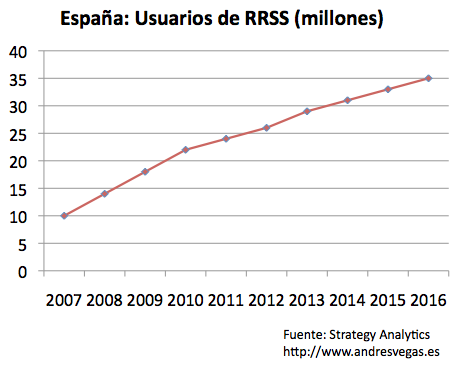
\includegraphics[width=0.75\textwidth]{imaxes/evorss.png}
	\caption{Evolución del uso de las redes sociales}
	\label{evorss}
\end{figure}

Este auge de las redes sociales no solo despierta la curiosidad de los empresarios, sino que también, y de forma muy ligada al interés económico inherente, nos permite disponer de un corpus muy extenso de textos que nos servirán como punto de partida para la construcción de un sistema clasificador.

Además de esto, cabe destacar el gran avance tecnológico realizado en los últimos años, permitiéndonos tener ordenadores cada vez más potentes, con unas capacidades de procesamiento tanto de CPU como de GPU altísimas y gracias a ello realizar entrenamientos con topologías mucho más complejas en un rango de tiempo menor. Es por esto que una de las ramas que hemos investigado para procurar una mejora del resultado final es una aproximación a las redes neuronales, las cuales se entrenan aprovechando la potencia de la GPU.

Hemos visto en este tipo de sistemas una oportunidad de negocio, ofreciendo al cliente ampliar su plataforma implementando un sistema de ranking automático de la lista de resultados mediante un pesado de la polaridad de las opiniones que los usuarios realizan sobre cada uno de los productos. De esta forma los usuarios podrán agilizar sus búsquedas, encontrando en los primeros lugares los elementos más relevantes, y el cliente podría realizar estudios sobre la aceptación de los mismos en el mercado.

\section{Objetivos}

El objetivo de esta investigación es el de analizar y comparar distintos modelos de clasificación de polaridades de textos utilizando procesamiento de lenguaje natural, para posteriormente utilizar estos modelos en la clasificación de comentarios realizados en una web de materiales de construcción.

Además se implementarán los módulos necesarios en una aplicación web para facilitar al usuario la publicación de estos comentarios.

\subsection{Análisis de sentimientos}

La tarea consiste en buscar una serie de características en el texto, en este caso comentarios, presumiblemente breves, sobre materiales de construcción, que nos ayude a realizar una clasificación de los mismos dividiéndolos en distintas clases.

Esta tarea es conocida como Análisis de Sentimiento (Das y Chen \cite{Das}, Tong \cite{Tong}, Turney \cite{Turney}, Pang et al. \cite{Pang}), Extracción de opiniones, Minería de Opiniones (introducido por Dave et al. \cite{Dave}), Minería de sentimiento o Análisis Subjetivo.

El ámbito de clasificación de esta tarea suele ser el siguiente:
\begin{itemize}
	\item Binario: El resultado se divide en dos clases bien diferenciadas (Opinión positiva y opinión negativa)
	\item Multiclase: El resultado se divide en 5 clases (Muy negativa, negativa, neutra, positiva, muy positiva)
	\item Tri-clase: El resultado se divide en 3 clases (Negativa, neutra y positiva)
\end{itemize}

Es de esperar que a mayor número de clases el problema se haga más complicado. Dado el dominio textual de la tarea es más difícil encontrar las diferencias entre un texto muy negativo y uno negativo que entre una opinión negativa y otra positiva.

Esta tarea suele resultar difícil incluso para humanos, ya que la valoración está fuertemente influenciada por valores subjetivos de cada observador. Por ejemplo la frase \emph{No me ha gustado la calidad del producto} podría ser considerada negativa por un observador imparcial y muy negativa por la persona responsable de la calidad de dicho producto.

El punto principal de la tarea es la extracción de características clave del texto que ayuden a separar y clasificar los textos en clases. En este área encontramos 2 aproximaciones principales:

\begin{itemize}
	\item Bag of words (BOW): Es el modelo más simple, se compone un vector de características en el que cada elemento se corresponde a una palabra del dominio, y su valor será o bien el número de ocurrencias en el texto o bien un valor estadístico que refleje la relación de la palabra con su contexto, como por ejemplo el valor de tf-idf.
	\item Word Embeddings (WE): Es un vector compuesto mediante un entrenamiento en una red neuronal que recibe como entrada un conjunto grande de textos e intenta aprender las relaciones de similitud entre las palabras que lo componen, dando como resultado para cada palabra un vector de dígitos reales de una longitud determinada. Gracias a este tipo de datos es posible buscar relaciones de similitud, o incluso operaciones de adición y sustracción entre los vectores que representan las palabras, dando como resultado otra palabra:
	\subitem Vector(Rey) - Vector(Hombre) + Vector(Mujer)  = Vector(Reina)
\end{itemize}


\subsection{Servicio web}
Pretendemos poner a disposición del usuario una web para realizar una búsqueda semántica de los productos, que además les ofrecerá un servicio de comentarios con las siguientes funcionalidades:

\begin{itemize}
	\item Añadir comentarios: Los usuarios podrán añadir nuevos comentarios tanto si están registrados como si son usuarios anónimos.
	\item Editar comentarios: Los usuarios registrados podrán editar sus comentarios.
	\item Borrar comentarios: Los usuarios registrados podrán eliminar sus comentarios.
\end{itemize}

Además el objetivo final de este servicio es clasificar los comentarios de manera que este resultado se pueda utilizar en un sistema de ranking de los resultados ofrecidos por el buscador semántico.

 
\chapter{Estructura de la memoria}

\lettrine{L}{a} memoria se estructurará en varios capítulos detallados a continuación:

\begin{itemize}
	\item \textbf{Introducción:} En este capítulo explicaremos la motivación y los objetivos del estudio, además de presentar la estructura de la memoria.
	\item \textbf{Estado del Arte:} Se definirán términos relativos al dominio del problema y se realizará un breve análisis de las investigaciones previas sobre el análisis de sentimientos.
	\item \textbf{Fundamentos tecnológicos:} Capítulo en el que se describirán las tecnologías y herramientas utilizadas para la implementación del proyecto.
	\item \textbf{Metodología de desarrollo:} Se explicará la metodología utilizada.
	\item \textbf{Planificación:} Se detallará la planificación llevada a cabo para afrontar el proyecto.
	\item \textbf{Análisis:} Definiremos las arquitecturas seleccionadas para el proyecto, comenzando por una definición de la arquitectura general y posteriormente detallando las arquitecturas propias de cada subsección del proyecto.
	\item \textbf{Casos de uso:} Apartado en el que se detallarán los casos de uso a abordar en la implementación del proyecto.
	\item \textbf{Implementación:} En este capítulo explicaremos la puesta en marcha del proyecto, explicando los detalles de la implementación tanto para el problema de clasificación como para el desarrollo del servicio web.
	\item \textbf{Resultados:} Análisis de los resultados obtenidos en los distintos experimentos.
	\item \textbf{Conclusiones:} Se tratará de llegar a una serie de conclusiones a partir de los resultados presentados previamente.
	\item \textbf{Solución desarrollada:} Apartado en el que se mostrará el resultado final del desarrollo.
\end{itemize}
 

\chapter{Estado del arte}

\lettrine{S}{on} muchos los estudios que se han publicado acerca del tema de la minería de opiniones. En esta investigación nos centraremos las técnicas más comunes de aprendizaje supervisado analizando distintos métodos tanto de clasificación como de preprocesamiento del texto.

En este capítulo describiremos el estado actual de los modelos de clasificación.

\section{Clasificación}
En términos de clasificación de sentimientos son muchos los trabajos publicados en los últimos tiempos (ver fig. \ref{pubsent}) debido a, como ya hemos comentado, el auge de las redes sociales y de la necesidad de las empresas por realizar un estudio de mercado y de satisfacción de sus clientes.

\begin{figure}[!ht]
	\centering
	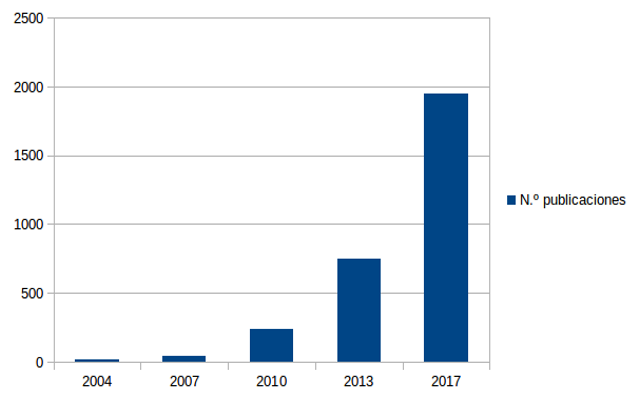
\includegraphics[width=0.75\textwidth]{imaxes/pubsentAnalisis.png}
	\caption{Publicaciones sobre Análisis de sentimientos en el IEEE desde 2004 hasta la actualidad}
		\label{pubsent}
\end{figure}

Dada la amplia extensión de métodos utilizados\footnote{http://www.sciencedirect.com/science/article/pii/S2090447914000550} para resolver este problema nosotros nos centraremos en las dos ramas utilizadas para el trabajo, utilizando un lexicón termino-sentimiento \cite{PabloG} y mediante algoritmos de aprendizaje automático, basándose la mayoría de estos estudios en los trabajos de Pang et al. \cite{Pang} intentando diseñar métodos más efectivos de extracción de características para mejorar la clasificación. En este último campo podríamos realizar una subdivisión atendiendo al tipo de algoritmo utilizado:

\begin{itemize}
	\item Machine Learning: Algoritmos tradicionales de aprendizaje supervisado, en los que se pretende obtener una matriz de características que servirán para extraer patrones que dividan los textos en distintas clases.
	\item Deep Learning: Se trata de algoritmos más novedosos, que están obteniendo alta relevancia en los últimos años (fig. \ref{pdeep}) gracias a la mejora de la capacidad de procesamiento de las GPU actuales. Estos modelos nos permiten obtener unos resultados mejores que los modelos tradicionales y además se ejecutan de forma más rápido gracias al alto rendimiento de las GPUs. 
	
	Además mediante esta rama de clasificación el vector de características se compone de Word Embeddings (WE) los cuales son mucho más ricos en información relacionada con la palabra que las features utilizadas en algoritmos tradicionales, ya que capturan información sobre similitud y características semánticas de las palabras.
	
	\begin{figure}[!ht]
		\centering
		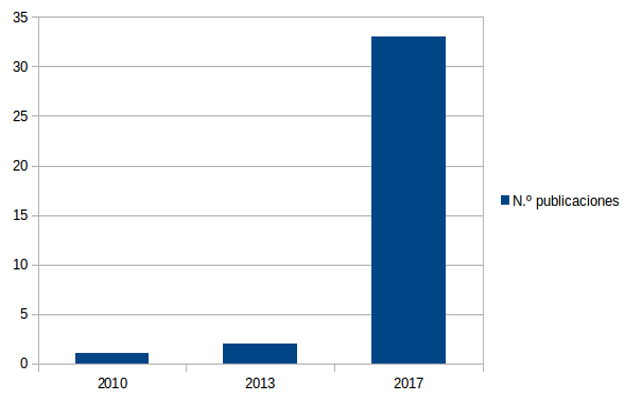
\includegraphics[width=0.75\textwidth]{imaxes/pubsDeep.png}
		\caption{Publicaciones en el IEEE desde 2010 que están relacionadas al término de búsqueda: sentiment analysis deep learning.}
				\label{pdeep}
	\end{figure}
\end{itemize}
Destacamos en esta sección los estudios realizados en la Universidad de Stanford \cite{Stanford}, obteniendo una precisión del 85.4\% para predicción binaria a nivel de oración.

\section {Conclusión}

Vistos los estudios anteriormente citados, vamos a realizar una implementación utilizando algoritmos típicos de Machine Learning que nos sirva como línea base, para posteriormente procurar mejorarla, tanto mejorando los procesos de tratamiento del texto como implementando modelos de Deep Learning.
 \chapter{Fundamentos Tecnológicos}
\lettrine{E}{n} este capítulo trataremos las distintas tecnologías utilizadas en el desarrollo de este proyecto.

\section{Análisis de sentimientos}

Para la preparación y estudio de los datos, así como para el desarrollo de los modelos de aprendizaje se ha elegido la versión 3.5 de Python, por su facilidad de aprendizaje y su amplia comunidad en el ámbito del aprendizaje automático.

Se trata de un lenguaje de programación multiparadigma creado por Guido van Rossum\footnote{https://docs.python.org/3/faq/general.html\#why-was-python-created-in-the-first-place} y administrado por la Python Software Foundation. 

Para el proyecto se han utilizado las siguientes librerías:


\begin{itemize}
	\item NLTK: Biblioteca para trabajar en dominios de lenguaje natural.
	\item SciKitLearn: Ofrece herramientas eficientes para el análisis y la minería de datos así como algoritmos de Machine Learning.
	\item TensorFlow: Biblioteca de código abierto para la implementación de modelos de Aprendizaje Profundo. Permite el uso tanto de CPU como de GPU durante los procesos. Se ha elegido esta frente a otras como Theano o Torch por ser una biblioteca de Google que sigue mantenida en la actualidad, permite su uso en contenedores Docker de forma que la instalación para el uso de GPU se simplifica y no afecta al sistema principal de la máquina. Además disfruta de una amplia comunidad de desarrolladores lo cual facilitará la resolución de dudas durante el proceso. 
	\item Keras: Biblioteca de alto nivel que permite agilizar la implementación de modelos de Aprendizaje Profundo. Está incluida de forma nativa en las últimas versiones de Tensorflow pero también se puede utilizar de forma individual con otros backends como Theano.
\end{itemize}


\section{Aplicación Web}

\subsection{Tecnología Back-end}
A continuación describiremos la tecnología utilizada del lado del servidor.

\subsubsection{Java}

El lenguaje de programación Java fue creado en 1991 por Sun Microsystems (adquirida posteriormente por Oracle) y publicado en 1995 como parte fundamental de la plataforma Java, que ofrece un lenguaje de programación de propósito general, concurrente y orientado a objetos.

La tecnología Java ofrece una máquina virtual (JVM) que permite ejecutar la compilación de los bytecodes (clases de Java) en cualquier máquina, sin importar la arquitectura subyacente.

Para la ejecución como usuario final de aplicaciones Java es necesario disponer del Java Runtime Environment (JRE), mientras que para el uso como desarrollador es necesario el uso del kit JDK (java Development Kit) que incluye el JRE.

Sun define tres plataformas según el entorno de aplicación:
\begin{itemize}
	\item Java ME: orientado a entornos de recursos limitados, como teléfonos móviles, PDAs, etc.
	\item Java SE: para entornos de gama media y estaciones de trabajo.
	\item Java EE: orientada a entornos distribuidos empresariales o de internet.
\end{itemize}

En el proyecto se utiliza la versión 8 del JDK con la plataforma Java EE.

\subsubsection{Spring}

Uno de los problemas a los que nos enfrentamos al enfrentarnos a un desarrollo software es el uso de varios frameworks (conjunto de clases que pretenden facilitarnos el trabajo), y cada uno de estos generará su propio conjunto de objetos. Esta situación puede generarnos problemas ya que los frameworks son independientes entre sí y gestionan ciclos de vida propios para los objetos.

En este sentido Spring nos ayuda cambiando las responsabilidades y encargándose él en lugar del desarrollador de generar los objetos de cada uno de los frameworks basándose en ficheros xml o anotaciones, y de integrarlos de forma correcta.

\subsubsection{Jackson}

Se trata de una biblioteca java simple pero potente pensada para serializar objetos Java a JSON y viceversa.

\subsection{Tecnología de datos}

A continuación se describen las tecnologías de gestión de datos utilizados por el sistema.

\subsubsection{PostgreSQL}
PostgreSQL es un sistema de gestión de base de datos relacional orientado a objetos y libre, publicado bajo la licencia PostgreSQL similar a la BSD o la MIT.

\subsubsection{Hibernate}

Hibernate es una herramienta de mapeado objeto-relacional (ORM) para uso sobre la plataforma Java o .Net bajo el nombre NHibernate.

Esta herramienta utiliza archivos XML o anotaciones en los beans de las entidades para facilitar el mapeado de atributos entre una base de datos relacional y el modelo de objetos de una aplicación.

\subsection{Front-end: Interfaz Single Page Application}

Una Single Page Application (SPA) es una aplicación o interfaz web de página única con el propósito de ofrecer una experiencia más fluida al usuario. Los códigos utilizados por la aplicación pueden cargarse todos de una sola vez o irse cargando de forma dinámica dependiendo de las necesidades de la aplicación.

Las herramientas modernas como AngularJS (que se explicará a continuación) permiten al desarrollador crear una SPA sin necesidad de enfrentarse al código JavaScript ni a los problemas de la tecnología. 

\subsubsection{HTML5}

HTML5 es la quinta revisión importante del lenguaje HTML y especifica dos variantes de sintaxis para HTML: una «clásica», HTML (text/html), conocida como HTML5, y una variante XHTML conocida como sintaxis XHTML5 que deberá servirse con sintaxis XML (application/xhtml+xml).

La versión definitiva de la quinta revisión del estándar se publicó en octubre de 2014.

\subsubsection{JavaScript}

Es un lenguaje de programación interpretado utilizado sobre todo del lado del cliente. Se define como orientado a objetos, basado en prototipos, imperativo, débilmente tipado y dinámico.

\subsubsection{CSS3}

CSS3 es la ultima versión disponible de CSS (Cacading Stylesheets u Hojas de estilo en cascada en Español). Cuando hablamos de CSS hablamos de un lenguaje de diseño gráfico que nos ayuda a suplir las carencias de HTML a la hora de maquetar el diseño de una página web.

\subsubsection{AngularJS}

AngularJS es un framework de javascript mantenido por Google que realiza una extensión del lenguaje HTML tradicional y nos brinda la posibilidad de diseñar páginas web dinámicas, facilitando la creación de SPA's.

Angular sigue el patrón MVVM (Model View View Model) alentando la articulación flexible entre la presentación, datos y componentes lógicos.

Se ha utilizado esta tecnología por ser la utilizada en el sistema ya existente, aunque sería recomendable hacer una migración a las nuevas versiones del framework.

\subsubsection{AngularMaterial}

Proyecto pensado para los desarrolladores de AngularJS que ofrece una serie de componentes prediseñados de interfaz siguiendo la especificación Google Material Design.

Las directivas y objetos ofrecidos por esta biblioteca están correctamente probados, y pensados para funcionar en diferentes dispositivos y a diferentes tamaños de pantalla (Responsive Web)

\subsubsection{JSPM}

JSPM es un gestor de paquetes asociado a SystemJS que funciona sobre cualquier registro como puede ser npm o GitHub y funciona sobre el sistema de carga de módulos ES6, característica que nos permite el uso de cualquier módulo javascript de forma sencilla, solo se necesita una instrucción para la instalación y una línea de código para la importación al proyecto.

Esta tecnología es la que utiliza el sistema existente, sin embargo si se migra a alguna de las últimas versiones del framework deberemos utilizar el gestor NPM.

\subsection{Tecnologías de despliegue y construcción}

\subsubsection{Servidor HTTP Apache}

Se trata de un servidor web de código abierto multiplataforma, que comenzó su desarrollo en 1995, actualmente es desarrollado y mantenido por una comunidad de usuarios bajo la supervisión de la Apache Software Foundation dentro del proyecto HTTP Server (httpd).

La estructura del servidor es modular, es decir, además de un core o núcleo presenta diversos módulos que aportan mucha funcionalidad que podría considerarse básica para un servidor web.

Además el servidor es fácilmente extensible incluyendo nuevos módulos además de los que trae por defecto.

\subsubsection{Apache Tomcat}

Tomcat es un contenedor web con soporte de servlets y JSPs. Incluye el compilador Jasper, que compila JSPs convirtiéndolas en servlets. El motor de servlets de Tomcat a menudo se presenta en combinación con el servidor web Apache.

\subsubsection{Apache Maven}

Maven es una herramienta de software para la gestión y construcción de proyectos Java creada por Jason van Zyl, de Sonatype, en 2002. 

Maven está construido alrededor de la idea de reutilización, y más específicamente, a la reutilización de la lógica de construcción. Como los proyectos generalmente se construyen en patrones similares, una elección lógica podría ser reutilizar los procesos de construcción.
 \chapter{Metodología de desarrollo}

\lettrine{E}{n} este capítulo describiremos la metodología elegida para la planificación y seguimiento del proyecto para posteriormente explicar sus características definitorias y las fases que lo componen, esto nos servirá como introducción para la explicación de la planificación realizada explicada en el capítulo \ref{sec:plani}.

\section{Proceso de desarrollo unificado}

El Proceso Unificado de Desarrollo Software o simplemente Proceso Unificado es un marco de desarrollo de software que se caracteriza por estar dirigido por casos de uso, centrado en la arquitectura y por ser iterativo e incremental. El refinamiento más conocido y documentado del Proceso Unificado es el Proceso Unificado de Rational o simplemente RUP.

\subsection{Características}

A continuación explicaremos las características que definen esta metodología.

\subsubsection{Iterativo e incremental}

El Proceso Unificado es un marco de desarrollo iterativo e incremental compuesto de cuatro fases denominadas Inicio, Elaboración, Construcción y Transición. Cada una de estas fases es a su vez dividida en una serie de iteraciones (la de inicio puede incluir varias iteraciones en proyectos grandes). Estas iteraciones ofrecen como resultado un incremento del producto desarrollado que añade o mejora las funcionalidades del sistema en desarrollo.

Cada una de estas iteraciones se divide a su vez en una serie de disciplinas:
\begin{itemize}
	\item Análisis de requisitos: En esta fase se analizan las necesidades de los usuarios finales del software para determinar qué objetivos debe cubrir. De esta fase surge una memoria llamada SRD (documento de especificación de requisitos), que contiene la especificación completa de lo que debe hacer el sistema sin entrar en detalles internos.
	\item Diseño: Descompone y organiza el sistema en elementos que puedan elaborarse por separado, aprovechando las ventajas del desarrollo en equipo. Como resultado surge el SDD (Documento de Diseño del Software)
	\item Implementación: Es la fase en donde se implementa el código fuente.
	\item Prueba: Los elementos, ya programados, se ensamblan para componer el sistema y se comprueba que funciona correctamente y que cumple con los requisitos, antes de ser entregado al usuario final.
\end{itemize}

\subsubsection{Dirigido por los casos de uso}

En el Proceso Unificado los casos de uso se utilizan para capturar los requisitos funcionales y para definir los contenidos de las iteraciones. La idea es que cada iteración tome un conjunto de casos de uso o escenarios y desarrolle todo el camino a través de las distintas disciplinas.

\subsubsection{Centrado en la arquitectura}

El Proceso Unificado asume que no existe un modelo único que cubra todos los aspectos del sistema. Por dicho motivo existen múltiples modelos y vistas que definen la arquitectura de software de un sistema.

\subsubsection{Enfocado a los riesgos}

El Proceso Unificado requiere que el equipo del proyecto se centre en identificar los riesgos críticos en una etapa temprana del ciclo de vida. Los resultados de cada iteración, en especial los de la fase de Elaboración deben ser seleccionados en un orden que asegure que los riesgos principales son considerados primero.

\subsection{Fases}

El PUD se puede dividir en cuatro fases que ayudaran tanto en la elaboración del software como a la resolución de problemas.

\subsubsection{Inicio}

En la fase de inicio se define el negocio: facilidad de realizar el proyecto, se presenta un modelo, visión, metas, deseos del usuario, plazos, costos y viabilidad.

\subsubsection{Elaboración}

En esta fase se obtiene la visión refinada del proyecto a realizar, la implementación iterativa del núcleo de la aplicación, la resolución de riesgos altos, nuevos requisitos y se ajustan las estimaciones.

\subsubsection{Construcción}

Esta abarca la evolución hasta convertirse en producto listo incluyendo requisitos mínimos. Aquí se afinan los detalles menores como los diferentes tipos de casos o los riesgos menores.

\subsubsection{Transición}

En esta fase final, el programa debe estar listo para ser probado, instalado y utilizado por el cliente sin ningún problema. Una vez finalizada esta fase, se debe comenzar a pensar en futuras novedades para la misma.

 \chapter{Planificación}\label{sec:plani}

\lettrine{A} continuación se detallan las fases seguidas en el proyecto, subdividiendo la gestión en las dos ramas principales del mismo: análisis de sentimientos y servicio web.

\section{Análisis de sentimientos}

\subsection{Fase 1: Inicio}

Se trata de una fase de documentación y aprendizaje.

En esta fase se realizará un análisis del estado del arte del problema, además se estudiará cuales son las tecnologías más comunes para abordarlo, y se tratará de familiarizarse con el dominio de la tarea.

\subsection{Fase 2: Elaboración}

Se establecen una serie de requisitos a cumplir por el clasificador, y se establecen los casos de uso. Posteriormente se realiza un primer modelado de la estructura de clases, que será posible que cambie según se vayan presentando nuevas posibilidades de experimentos a realizar.

\subsection{Fase 3: Construcción}

Se comienza la implementación del código, esta fase constará de varias iteraciones que irán sumando funcionalidades al sistema.

\paragraph{Iteración 1} En esta iteración se comenzará por la implementación de un algoritmo de clasificación que sirva como línea base. Además será necesario implementar el algoritmo de tratamiento del corpus de documentos, será necesario pasar de formato XML a un formato que sea válido como entrada de los clasificadores, en este caso se ha elegido un tipo DataFrame de Python, que nos facilitará el tratamiento posterior de los textos.

\paragraph{Iteración 2} Se procederá a implementar la clase de preprocesamiento de los textos que nos servirá para probar métodos para aumentar la eficacia del clasificador.

\paragraph{Iteración 3} Se desarrollarán una serie de estudios sobre los datos y las posibilidades de mejora tanto del preprocesado como de los algoritmos, partiendo de los resultados de la línea base.

\paragraph{Iteración 4} Se creará una clase capaz de procesar los resultados, y ofrecer recursos visuales de valor que nos ayuden a comparar los resultados obtenidos. 

\subsection{Fase 4: Fase de transición}
Con el programa listo se procederá a realizar las ejecuciones de los modelos y obtener unos datos que servirán para hacer una comparativa de los mismos. Como consecuencia de estos resultados se decidirá si es necesario corregir errores, buscar nuevos modelos o consideramos que el programa está ya listo para su entrega.

Es posible que tras finalizar esta fase veamos necesario volver a la fase anterior, ya sea por necesidad de corregir errores, o porque durante la investigación se ha descubierto alguna otra estrategia que se estime pueda funcionar mejor que la adoptada hasta ahora.

\section{Servicio web}

\subsection{Fase 1: Fase de inicio}
Dado que abordaremos la implementación de una sección de una página Web perteneciente a un proyecto ya existente, en esta primera fase trataremos de comprender el funcionamiento y la estructuración del código ya existente, posteriormente se hará un análisis de los requisitos del módulo.

\subsection{Fase 2: Fase de elaboración}

Tras haber comprendido el sistema existente y haber refinado los requisitos, procederemos a la extracción de los casos de uso, del modelo de base de datos y del modelado de clases.

\subsection{Fase 3: Fase de construcción}

Con toda la documentación establecida se procederá a la implementación de las funcionalidades del módulo siguiendo un ciclo de iteraciones.

\paragraph{Iteración 1} Se implementará en el servidor las operaciones CRUD\footnote{CRUD: Create Read Update Delete} de la entidad Comentario, así como los endpoints que permitirán al cliente acceder a estos servicios.

\paragraph{Iteración 2} Se creará la vista principal del módulo de comentarios que permitirá al usuario acceder a una lista de los mismos desde el perfil de cada producto.

\subsection{Fase de transición}

Se realizarán las pruebas finales para verificar que el módulo funciona tal y como se establece en los requisitos y que todos los casos de uso están implementados de forma correcta.

\section{Diagrama de Gantt}

\begin{figure}[!ht]
	\centering
	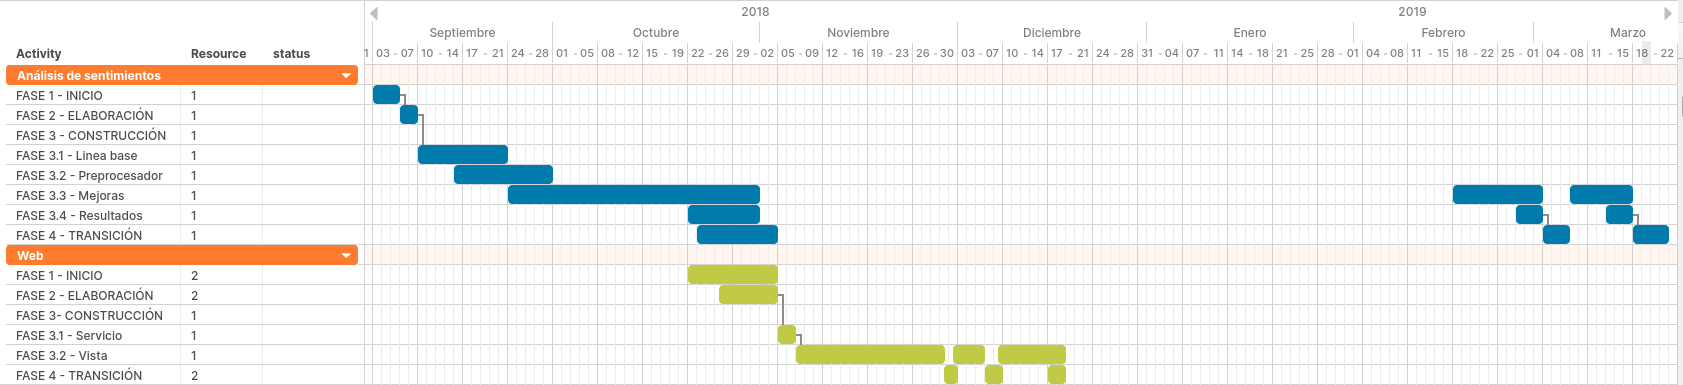
\includegraphics[width=1\textwidth]{imaxes/gantt.png}
	\caption{Diagrama de Gantt del proyecto (BCS).}
	\label{gant}
\end{figure}

El diagrama de Gantt realizado para el proyecto (fig. \ref{gant}) representa los tiempos de desarrollo en un BCS (Best Case Scenario).

En esta casuística el proyecto podría durar hasta 4 meses de desarrollo como mínimo, aunque en el diagrama se incluye la posibilidad de encontrar algún fallo o método de clasificación más eficaz meses más tarde.

Como vemos las tareas no tienen por qué ser secuenciales, dado que si suponemos que la carga prevista de la tarea va a ser baja podemos paralelizarla con otra, y en muchos casos la propia naturaleza de la tarea nos obligará a ejecutarla de forma paralela, ya que, por ejemplo la construcción del preprocesador de textos se verá influida por los resultados obtenidos en la clasificación y viceversa.

En cuanto a la parte final del desarrollo web vemos que se intercalan la fase 4 y la fase 3.2, esto se debe a que esperamos encontrar fallos en las fases de prueba que necesitarán ser corregidos y probados de nuevo.

En el desarrollo real de este proyecto se ha entregado el PVM (Producto Viable Mínimo) dentro del tiempo especificado en la estimación. Sin embargo se han realizado varios ciclos de desarrollo posteriores para mejorar la implementación de ciertos algoritmos, mediante prueba de nuevas tecnologías, corrección de errores o afinación de hiperparámetros. Estos esfuerzos sumarán un total de 192 horas imputables a las tareas 3.3 y 3.4 del análisis de sentimientos.

\section{Estimación de recursos}

Para la realización de este proyecto se necesitarán al menos 2 personas con 2 roles diferenciados, un analista que se encargue de la recogida de requisitos y diseño inicial del sistema y un programador que lo implemente.

En caso de ser necesario podríamos recurrir a un tercer recurso para la realización de la investigación, que bien podría ser un ingeniero de datos o un especialista en el campo del aprendizaje automático.

\section{Estimación de costes}

Para realizar la estimación de costes vamos a tener en cuenta la participación de dos recursos, un analista en las fases iniciales del desarrollo web y un programador junior a lo largo de todo el proyecto. Los cálculos se realizarán sobre la estimación inicial, sin tener en cuenta el tiempo de desarrollo fuera del escenario BCS.

Los recursos tendrían una remuneración de:

\begin{itemize}
	\item Analista: 17€/hora
	\item Programador: 12€/hora
\end{itemize}

A continuación se muestran las tablas con la estimación de esfuerzo de los recursos durante los tres meses y medio estimados como mejor escenario posible, separadas por subsitemas.

\begin{table}[H]
	\centering
\begin{tabular}{|l|c|c|c|}
	\hline
	Tarea  & Precio (€/hora) & Esfuerzo aprox. (horas) & Total (€) \\ \hline
	FASE 1 & 12              & 24                      & 288       \\ \hline
	FASE 2 & 12              & 16                      & 192       \\ \hline
	FASE 3 & 12              & 384                      & 3072       \\ \hline
	&                 & 424 h                    & 3552 €    \\ \hline
\end{tabular}
\caption{Estimación de esfuerzo subsistema de análisis de sentimientos.}
\label{esf-anal-sent}
\end{table}

\begin{table}[H]
	\centering
	\begin{tabular}{|l|c|c|c|}
		\hline
		Tarea  & Precio (€/hora) & Esfuerzo aprox. (horas) & Total (€) \\ \hline
		FASE 1 & 17              & 80                      & 1360      \\ \hline
		FASE 2 & --              & 56                      & --        \\ \hline
		FASE 3 & 12              & 256                     & 3072      \\ \hline
		&                 & 336 h                   & 4432 €    \\ \hline
	\end{tabular}
\caption{Estimación de esfuerzo desarrollo aplicación web.}
\label{esf-web}
\end{table}

Como vemos en la tabla \ref{esf-web} en las primeras fases solo se ha tenido en cuenta el trabajo realizado por el analista, ya que el programador tendrá que paralelizar esta etapa con la fase final del otro subsistema. Además dado que el analista paralelizará su trabajo en estas primeras fases la fase 2 de 56 horas no supondrá un costo a mayores.

Teniendo estos datos en cuenta podemos estimar un coste de 7.984 € para el proyecto. Si además sumamos el costo de las 192 horas asignadas al programador para un posible caso de arreglo o mejora futura obtenemos un total de 10.288€.





 
\chapter{Casos de uso}\label{chap:cu}

\lettrine{D}{urante} este capítulo se presentarán los diversos casos de uso que han de ser implementados en la aplicación.

\begin{figure}[!ht]
	\centering
	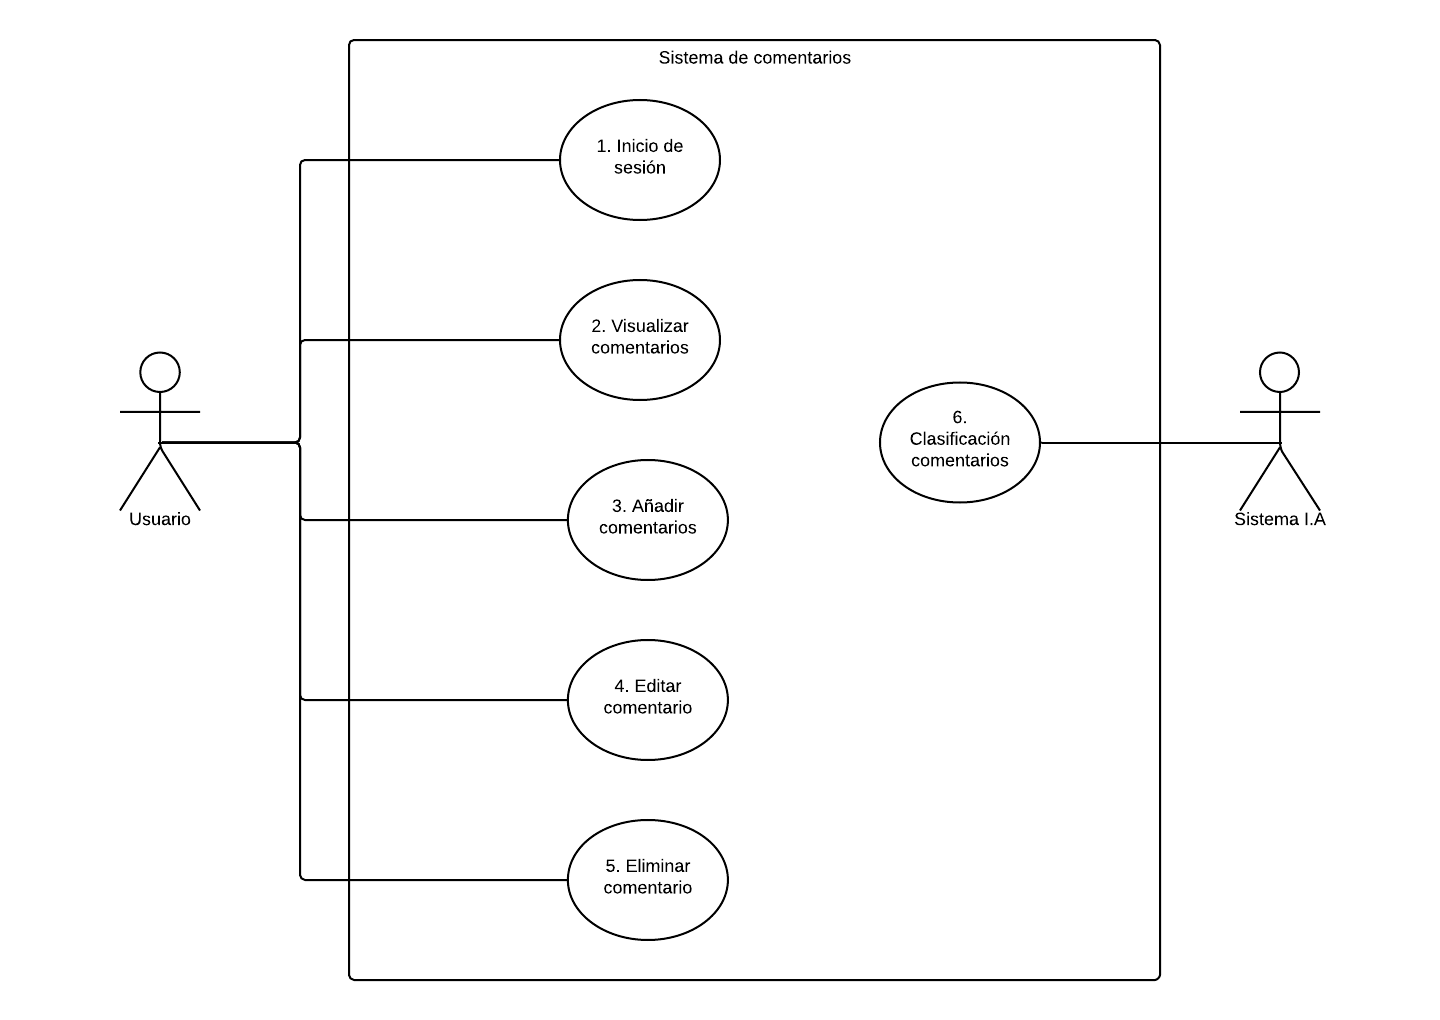
\includegraphics[width=1\textwidth]{imaxes/usecases.png}
	\caption{Casos de uso}
		\label{usecases}
\end{figure}

\section{Inicio de sesión}

\paragraph{Descripción} El usuario iniciará sesión en la aplicación introduciendo sus credenciales en un formulario.

\paragraph{Precondición} El usuario está dado de alta en el sistema

\paragraph{Secuencia} La secuencia de acciones será la siguiente:

\begin{itemize}
	\item El usuario pulsa el botón de inicio de sesión.
	\item El usuario introducirá sus credenciales en el formulario.
	\item Si las credenciales son correctas se notifica al usuario de que su sesión se ha iniciado y se cambia el botón de inicio de sesión por el botón de gestión de perfil.
	\item Si las credenciales no son correctas se notifica al usuario y se vuelve a pedir que las introduzca de nuevo.
\end{itemize}

\paragraph{Postcondición} La sesión del usuario quedará iniciada en el sistema.

\section{Visualizar comentarios}

\paragraph{Descripción} El usuario visualizará los comentarios de un artículo cuando abra la ficha del mismo haciendo click sobre el mismo en la pantalla principal.

\paragraph{Precondición} El articulo debe estar registrado en el sistema.

\paragraph{Secuencia} El caso de uso comenzará cuando el usuario haga click sobre un artículo determinado en la rejilla de resultados de búsqueda.

\section{Añadir comentarios}

\paragraph{Descripción} El usuario podrá añadir comentarios relacionados con alguno de los artículos del sistema.

\paragraph{Precondición} El articulo debe estar registrado en el sistema.

\paragraph{Secuencia} La secuencia de acciones será la siguiente:

\begin{itemize}
	\item 1 El usuario hace click sobre alguno de los artículos de la rejilla de resultados de la página principal.
	\item 2 El usuario introduce el comentario que desee en el cuadro de texto.
	\item 3 El usuario puede publicar o cancelar el comentario.
	\SubItem{3.1 Si el usuario introduce una puntuación para el artículo esta se le asigna al comentario.}
	\SubItem{3.2 Si el usuario no introduce una puntuación el artículo se guardará sin puntuación asociada, y se le asignará mediante un modelo de clasificación inteligente.}
	\SubItem{3.3 Si el usuario cancela el envío del comentario se terminará el caso de uso.}
\end{itemize}
	
\paragraph{Postcondición} El comentario quedará dado de alta en el sistema y asociado al artículo correspondiente.


\section{Editar comentarios}

\paragraph{Descripción} El usuario podrá editar los comentarios realizados con anterioridad.

\paragraph{Precondición} 
\begin{itemize}
	\item El usuario debe estar registrado.
	\item El comentario a editar debe pertenecer al usuario.
\end{itemize}

\paragraph{Secuencia} La secuencia de acciones será la siguiente:

\begin{itemize}
	\item 1 El usuario hace click sobre alguno de los artículos de la rejilla de resultados de la página principal.
	\item 2 El usuario elige la opción de edición sobre uno de sus comentarios.
	\item 3 El usuario puede aplicar o cancelar la edición.
	\SubItem{3.1 Si el usuario introduce una puntuación para el artículo esta se le asigna al comentario.}
	\SubItem{3.2 Si el usuario no introduce una puntuación el artículo se guardará sin puntuación asociada, y se le asignará mediante un modelo de clasificación inteligente.}
	\SubItem{3.3 Si el usuario cancela el envío del comentario se terminará el caso de uso.}
\end{itemize}

\paragraph{Postcondición} El comentario quedará modificado en el sistema.


\section{Eliminar comentarios}

\paragraph{Descripción} El usuario podrá eliminar los comentarios realizados con anterioridad.

\paragraph{Precondición} 
\begin{itemize}
	\item El usuario debe estar registrado.
	\item El comentario a eliminar debe pertenecer al usuario.
\end{itemize}

\paragraph{Secuencia} La secuencia de acciones será la siguiente:

\begin{itemize}
	\item 1 El usuario hace click sobre alguno de los artículos de la rejilla de resultados de la página principal.
	\item 2 El usuario elige la opción de eliminar sobre uno de sus comentarios.
	\item 3 El sistema pedirá confirmación antes de realizar el borrado.
	\SubItem{3.1 Si el usuario acepta la eliminación se borrará el comentario del sistema.} 
	\SubItem{3.2 Si el usuario no confirma la eliminación se termina el caso de uso.}
\end{itemize}
	
\paragraph{Postcondición} El comentario quedará borrado del sistema.

\section{Clasificar comentarios}

\paragraph{Descripción} El sistema puntuará los nuevos comentarios según la opinión reflejada en los mismos.

\paragraph{Precondición} 
\begin{itemize}
	\item Hay nuevos comentarios en el sistema o hay un nuevo modelo de clasificación.
\end{itemize}

\paragraph{Secuencia} La secuencia de acciones será la siguiente:

\begin{itemize}
	\item 1 Si hay un nuevo modelo de clasificación:
	\SubItem{1.1 Se obtienen todos los comentarios.}
	\SubItem{1.2 Se clasifican los comentarios obtenidos.}
	\SubItem{1.3 Se actualiza la clasificación de los comentarios en el sistema.}
	\item 2 Si hay nuevos comentarios:
	\SubItem{2.1 Se obtienen los nuevos comentarios.}
	\SubItem{2.2 Se clasifican los comentarios obtenidos.}
	\SubItem{2.3 Se actualiza la clasificación de los comentarios en el sistema.}
\end{itemize}
	
\paragraph{Postcondición} Todos los comentarios tienen una clasificación asociada.

 \chapter{Análisis}
\section{Arquitectura general}


\begin{figure}[!ht]
	\centering
	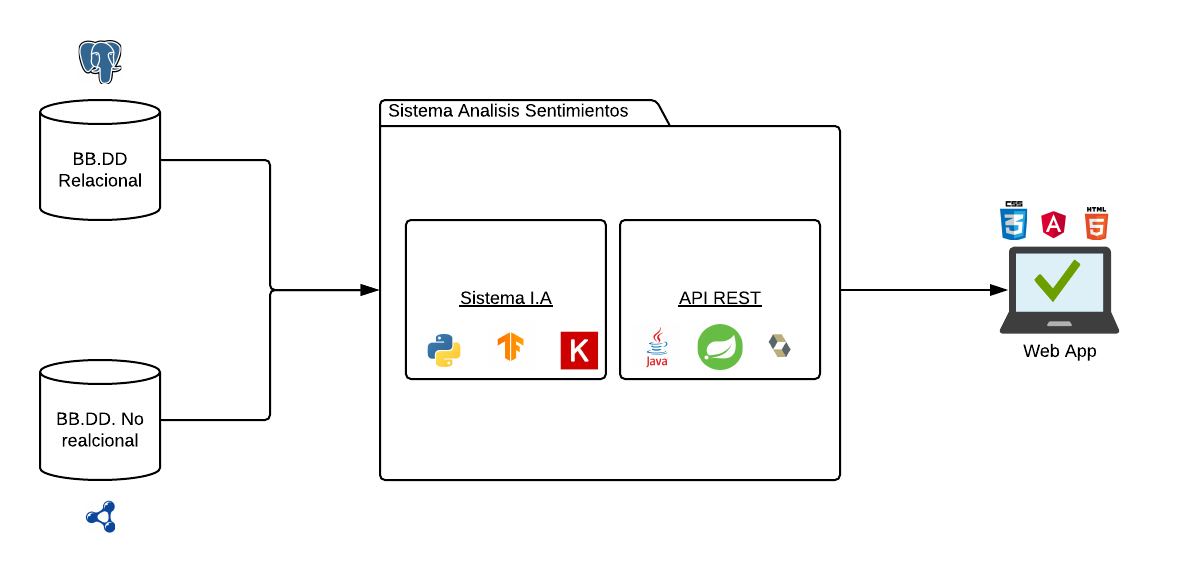
\includegraphics[width=1\textwidth]{imaxes/arqGeneral.png}
	\caption{Arquitectura general del sistema}
	\label{arqGen}
\end{figure}

Como vemos en la figura anterior el sistema se compone de un componente principal que incluye el sistema de inteligencia artificial (clasificación de comentarios) y un sistema que publica una API rest para poder comunicarse con los usuarios finales a través de una aplicación web.

Este sistema se vale de dos bases de datos:
\begin{itemize}
 \item BB.DD relacional: Se almacenan datos de artículos, usuarios y comentarios de forma que se puedan relacionar entre sí.
 \item BB.DD no relacional: Se trata de una base de datos documental con datos sobre las características de los artículos como el color o el material. Se almacena en forma de tripletas RDF y se utiliza en el proceso de búsqueda, el cual queda fuera del alcance de esta memoria.
\end{itemize}

\section{Arquitectura sistema de análisis de sentimientos}

\begin{figure}[H]
	\centering
	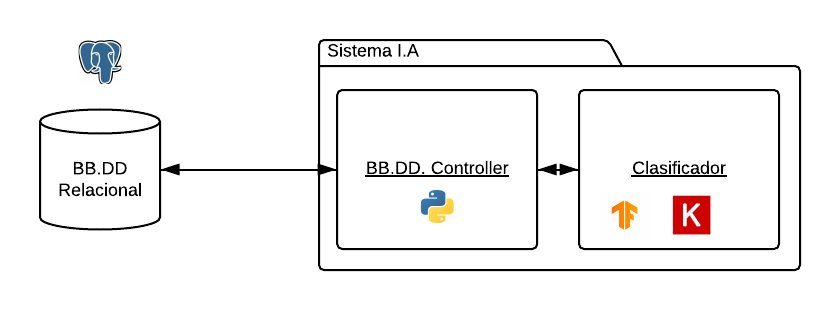
\includegraphics[width=1\textwidth]{imaxes/arqAI.png}
	\caption{Arquitectura del sistema de análisis de sentimientos}
	\label{arqAI}
\end{figure}

\begin{figure}[H]
	\centering
	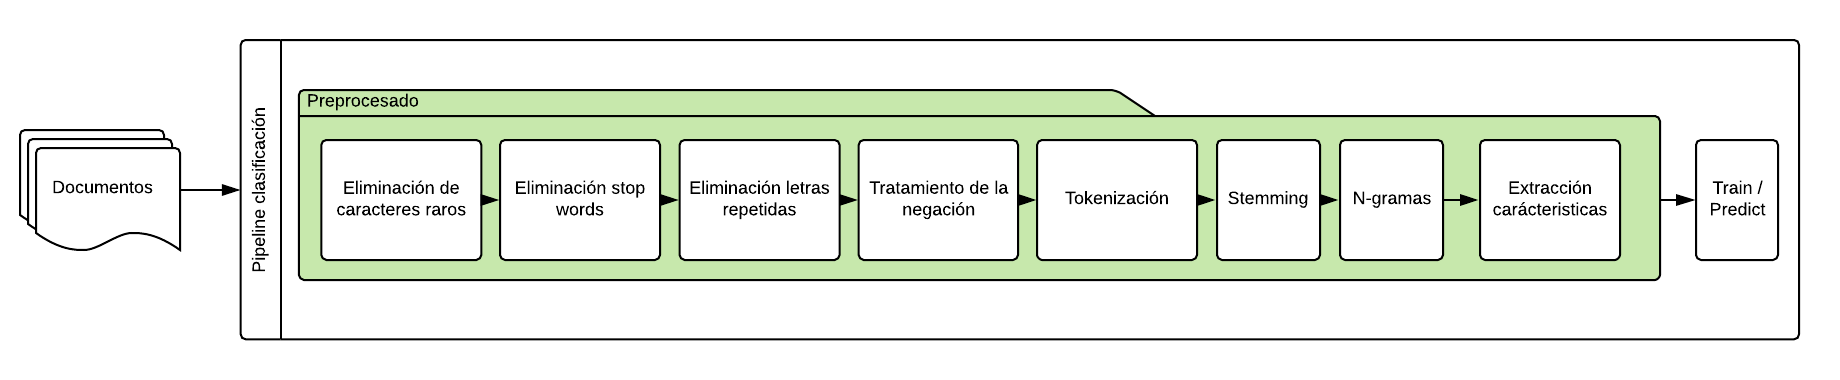
\includegraphics[width=1\textwidth]{imaxes/pipeclasif.png}
	\caption{Arquitectura del clasificador}
	\label{clasifPipe}
\end{figure}

El sistema de clasificación de comentarios (\ref{arqAI}) se compone de dos módulos:

\begin{itemize}
\item Un módulo para gestionar la obtención y actualización de comentarios con la base de datos.
\item Un módulo para realizar la clasificación (\ref{clasifPipe}): Compuesto por un pipeline con dos pasos principales, preprocesado y clasificación o entrenamiento. Los pasos del preprocesado no serán obligatorios y deberán activarse o desactivarse según lo que resulte más conveniente para obtener unos mejores resultados.
\end{itemize}

\section{Arquitectura Web}

\begin{figure}[H]
	\centering
	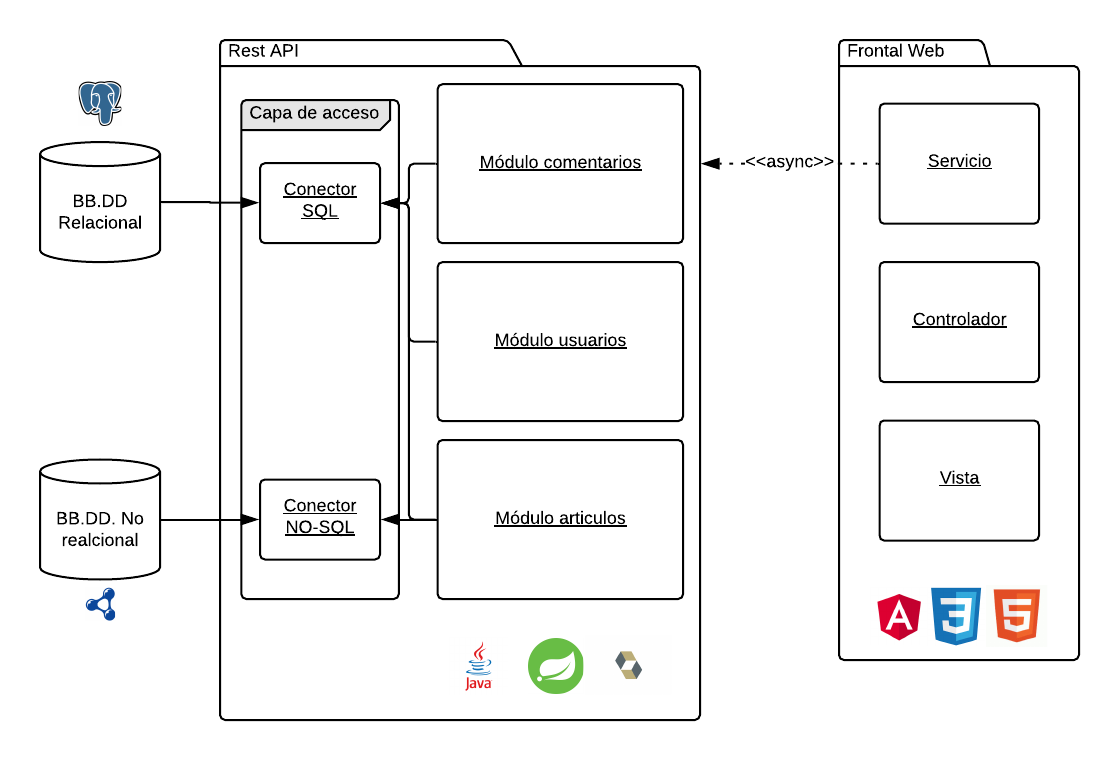
\includegraphics[width=1\textwidth]{imaxes/arqServ.png}
	\caption{Arquitectura del servicio y frontal web.}
	\label{arqServ}
\end{figure}

\begin{figure}[H]
	\centering
	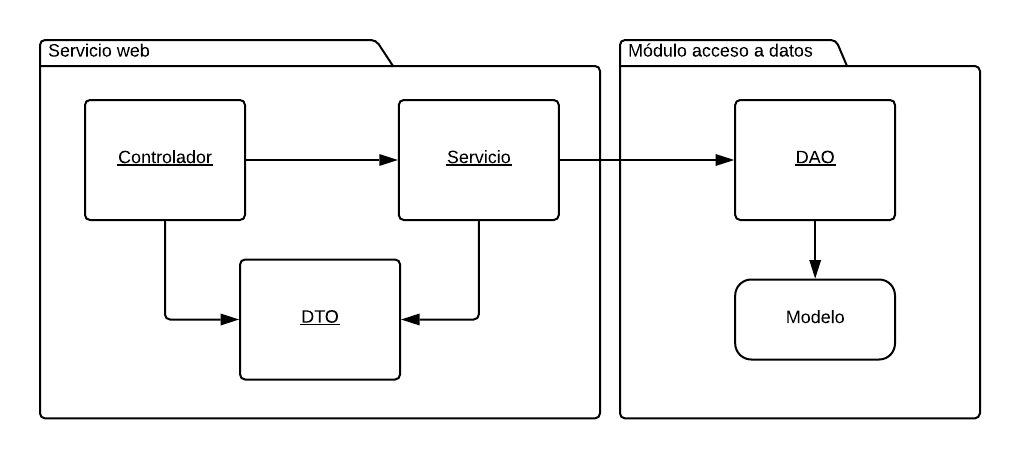
\includegraphics[width=0.75\textwidth]{imaxes/restmodel.png}
	\caption{Ejemplo de arquitectura de un módulo REST del servicio.}
	\label{restModel}
\end{figure}

La aplicación REST (\ref{arqServ}) se compone de tres módulos diferenciados para gestionar las distintas entidades del sistema: usuarios, artículos y comentarios.

Cada módulo sigue un patrón de acceso a datos DAO para abstraerse de la tecnología de base datos utilizada y ser más resistente a cambios, y un patrón DTO para la transmisión de datos, esto nos ayuda a reducir la cantidad de llamadas realizadas al sistema y permite al servicio web abstraerse de la implementación del back-end.

El frontal web se estructura con un patrón MVC (Modelo-Vista-Controlador) en el que el servicio realiza las llamadas asíncronas al API REST y devuelve los datos al controlador, que se encargará de la comunicación entre las vistas y los servicios.

\section{Trabajo futuro} Esta arquitectura se podría simplificar utilizando la nueva librería de javascript TensorflowJS. Con esto podríamos eliminar el sistema de clasificación de comentarios, clasificándolos en caliente en el momento de su publicación desde la aplicación WEB. 
Para utilizar esta librería solo necesitamos tener un modelo guardado en formato .h5, y dado que la clasificación es un proceso ligero no se espera que suponga una carga importante para el usuario final.

 \chapter{Base de datos}
\lettrine{E}{n} este capítulo trataremos el diseño de las tablas de base de datos en las que se persistirán los comentarios realizados por los usuarios, así mismo se representarán y describirán todas las entidades relacionadas con los mismos.

\section{Diseño lógico: Modelo Entidad-Relación}
A continuación, se muestra el modelo ER del sistema de comentarios. En este diagrama (fig. \ref{erDiag}) se representan las relaciones y atributos de las 3 entidades utilizadas en subsistema de comentarios: Usuario, Comentario y Articulo.

\begin{figure}[ht!]
	\centering
	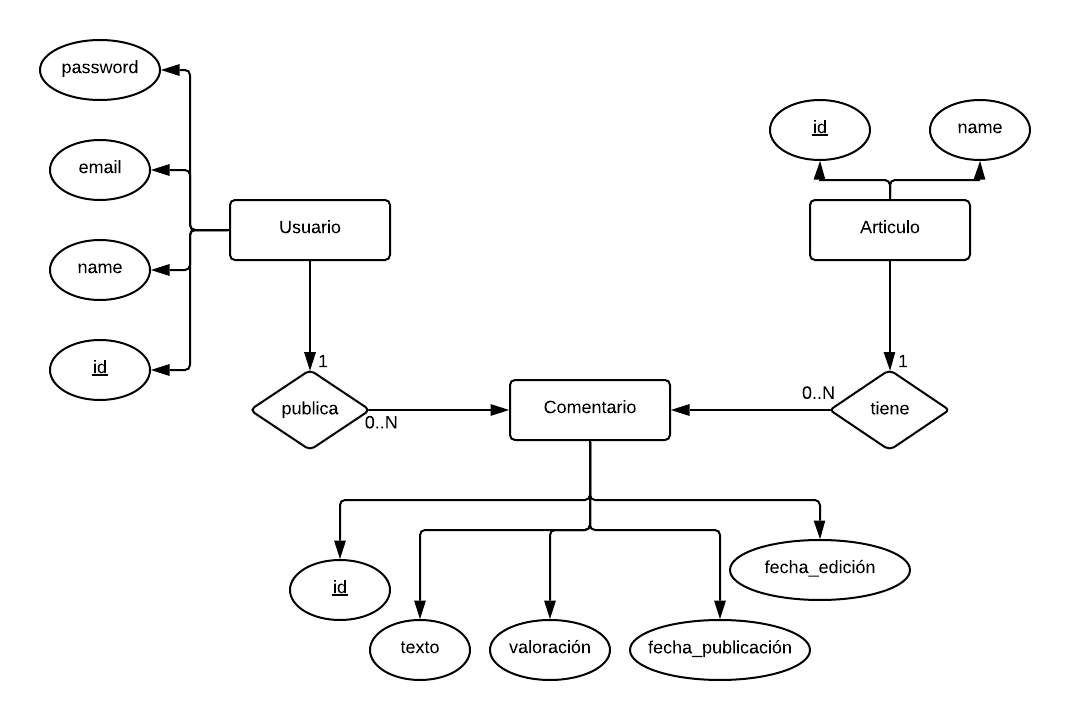
\includegraphics[width=1\textwidth]{imaxes/er.png}
	\caption{Diagrama entidad relación para el subsistema de comentarios.}
	\label{erDiag}
\end{figure}

Siguiendo los requisitos mínimos expuestos por el cliente, un usuario podrá publicar de 0 a N comentarios acerca de un producto, y cada articulo podrá tener 0 o N comentarios.

\section{Diseño físico: Modelo relacional}

La figura \ref{erModel} representa el modelo relacional del subsistema de comentarios.

\begin{figure}[ht!]
	\centering
	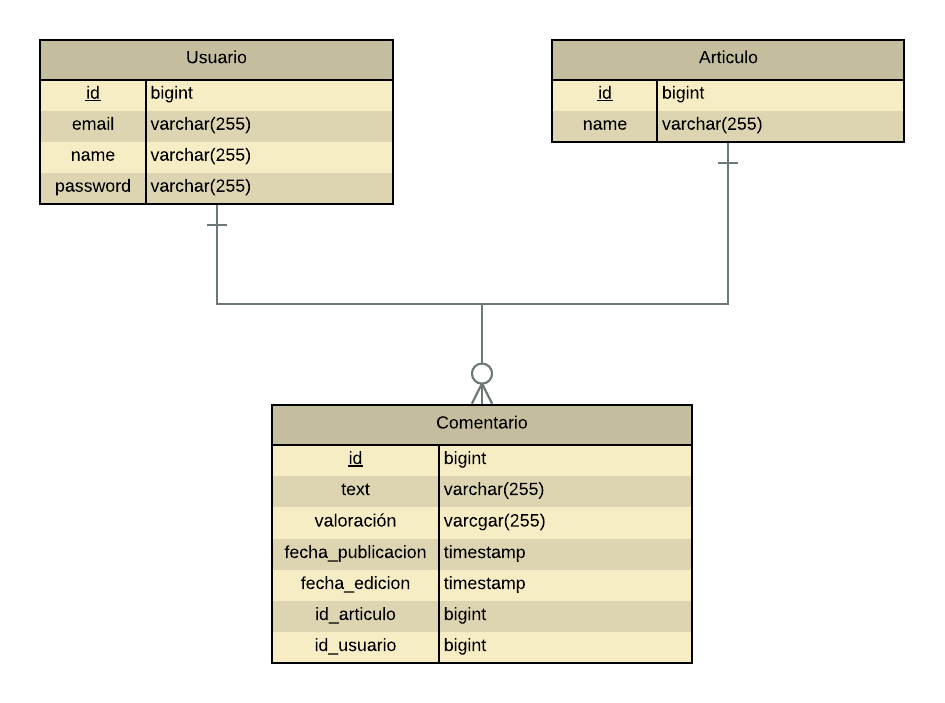
\includegraphics[width=0.75\textwidth]{imaxes/ermodel.png}
	\caption{Modelo relacional para el subsistema de comentarios.}
	\label{erModel}
\end{figure}
 
\chapter{Diseño}

\lettrine{E}{n} este capítulo describiremos la estructura de clases de los dos sistemas realizados en este trabajo.

\section{Análisis de sentimientos}

El sistema de análisis de sentimientos estará compuesto por una supercalse Classificator que contendrá métodos y parámetros comunes a las clases Machine Learning y Deep Learning. Estás dos subclases implementarán de forma individual el comportamiento de los métodos de entrenamiento y predicción. Para realizar el preprocesado de los documentos se creará la clase VectorizerHelper que extenderá de las clases de la biblioteca sklearn BaseEstimator y TrasformerMixin, esto nos permitirá utilizar esta clases como parte del pipe de la búsqueda de parámetros.

\subsection{Diagrama de clases}

\begin{figure}[H]
	\centering
	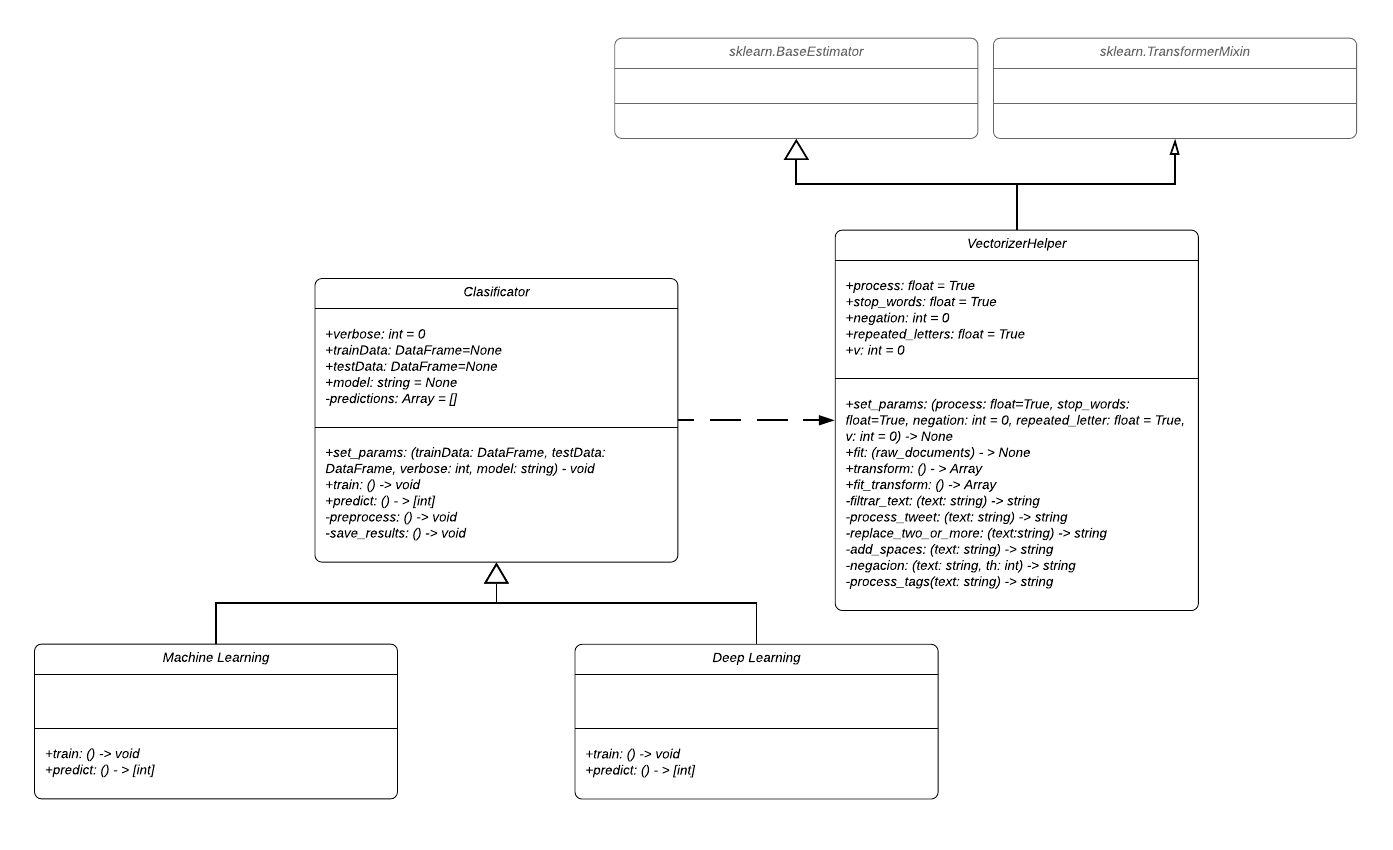
\includegraphics[width=1\textwidth]{imaxes/saClases.png}
	\caption{Diagrama de clases del sistema de análisis de sentimientos}
	\label{saClases}
\end{figure}

\section{Servicio web}

En esta sección se mostrará el diagrama de clases del servicio de comentarios. En la figura \ref{entClases} vemos la relación de las clases entidad relacionadas al comentario. En la figura \ref{daoClases} se describe la estructura del controlador y el servicio de comentarios, así como la descripción del DTO (Data Transfer Object) devuelto por el servicio. 

\subsection{Diagrama de clases}

\begin{figure}[H]
	\centering
	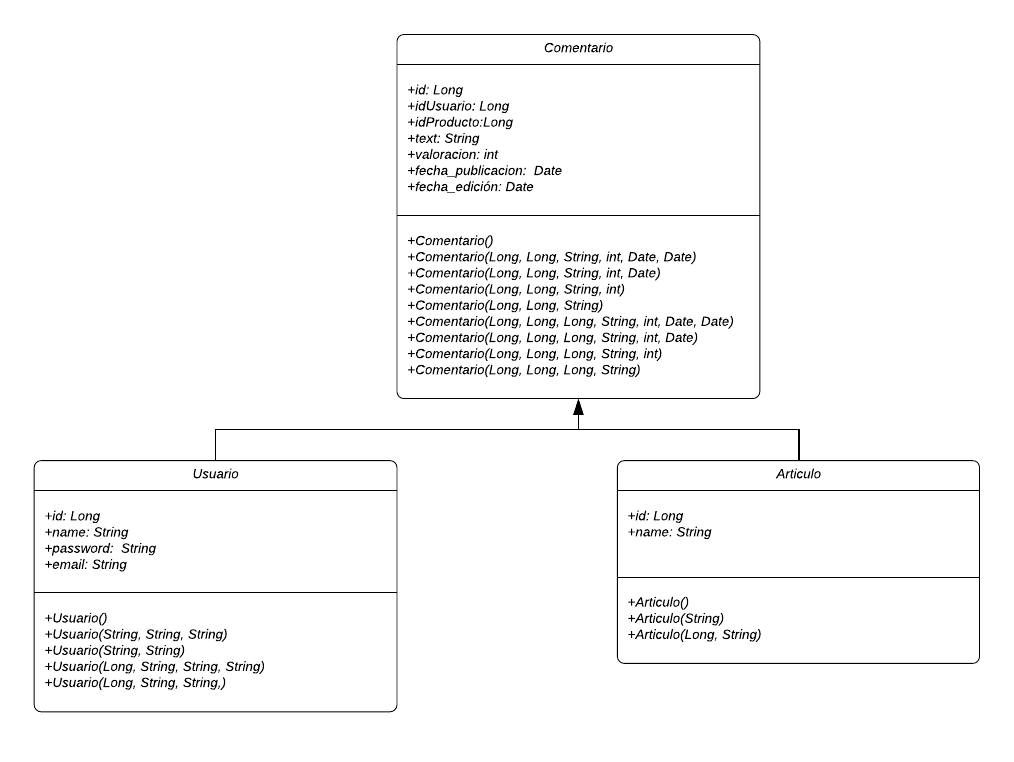
\includegraphics[width=0.75\textwidth]{imaxes/entClases.png}
	\caption{Diagrama de clases de las entidades del modelo SQL}
	\label{entClases}
\end{figure}

\begin{figure}[H]
	\centering
	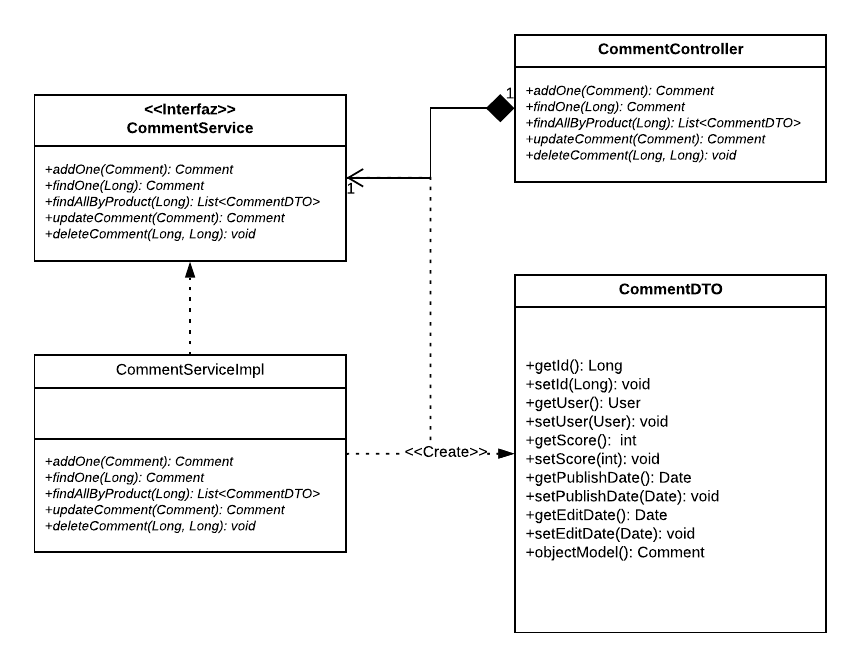
\includegraphics[width=0.70\textwidth]{imaxes/daoClases.png}
	\caption{Diagrama de clases de comentario.}
	\label{daoClases}
\end{figure}
 \chapter{Implementación}

\section{Análisis de sentimientos}

\subsection{Tratamiento de los datos}

Para poder realizar un trabajo de análisis de sentimientos es necesario llevar a cabo un proceso previo conocido como preprocesado con la intención de reducir la dimensionalidad del problema, y facilitar la tarea de clasificación de los algoritmos.

Los corpus de datos utilizados para las tareas de clasificación (ver sección \ref{corpus}) presentan mucho ruido,  además de palabras que no tienen un impacto real en la polarización del texto. Si tenemos en cuenta que los algoritmos de clasificación utilizan palabras como característica base para la clasificación, podemos ver que mantener estos elementos en los textos aumentará la dimensionalidad del problema, por lo tanto plantemos una serie de pasos que ayudarán a limpiar los textos como la eliminación de caracteres raros, tratamiento de emoticonos, eliminación de "stopwords", tratamiento de la negación, etc. Pasos de los cuales hablaremos en profundidad en este apartado.

El tratamiento de los datos se divide en dos grandes pasos principales: transformación y filtrado, mientras el proceso de transformación hace referencia a la adaptación del contenido de los textos, el filtrado se centra más en la reducción de la dimensionalidad de los mismos ya sea mediante métodos estadísticos (TF-IDF), mediante la identificación de la categoría morfológica de la palabra y eliminación de las menos significantes o la eliminación de "stopwords".

\subsubsection{Tokenización}

La tokenización es el paso base del preprocesado de textos, este paso consiste en la división del texto en sus átomos más básicos (palabras), que se conocen como tokens. Por ejemplo el texto \textit{ Es la mejor pelicula de mi vida } daría como resultado:

\begin{itemize}
	\item \textbf{tokens}: [Es, la, mejor, pelicula, de, mi, vida]
\end{itemize}

Estos tokens son utilizados como entrada del resto de procesos de los que hablamos en esta sección.

\subsubsection{Eliminación caracteres raros}

Dado que los textos proceden de entornos online es común encontrar en ellos elementos como URL, e-mails, abreviaturas, hashtags, nominaciones a usuarios (@usuario) o caracteres raros como signos de puntuación, corchetes, exclamaciones, etc. Estos elementos no aportan información importante a la hora de realizar una clasificación de los textos por lo que los eliminaremos de los mismos o los substituiremos por elementos que sí puedan aportar, como en el caso de algunas abreviaturas. Para entender el por qué de la substitución de abreviaturas hay que tener en cuenta que en el proceso de filtrado se escogen las palabras con más presencia en los documentos, por lo que si en algunos documentos aparece la palabra "gracias" que puede aportar un sentimiento positivo al mismo y en otros aparece la palabra "thx" de la abreviatura de la palabra inglesa "thanks", podemos encontrarnos un caso de disolución de la relevancia de la misma y que termine por no utilizarse como elemento del clasificador. 

\subsubsection{Eliminación letras repetidas}

Se ha comprobado que es muy frecuente en los documentos utilizados en nuestro sistema el uso abusivo de caracteres repetidos como forma de enfatizar un sentimiento o representar una forma de exageración.

\textit{ que maaaaaaaaalo!!!!! } 

Aunque esto resulte fácilmente interpretable para el lector humano, el sistema de aprendizaje automático no obtendrá ninguna conclusión de la aparición de estos elementos a menos de que un experto prepare los datos previamente creando algún tipo de constructo que el sistema pueda interpretar, o bien eliminándolos y reemplazándolos por una aparición única del elemento.

\textit{ que malo! } o \textit{ que muy malo }

\subsubsection{Tratamiento emoticonos}

Es común para el usuario de la red utilizar emoticonos o abreviaturas para expresar sus emociones en determinados momentos o contextos en los que se realice el comentario.

Para que el sistema interprete correctamente estos elementos es necesario crear un diccionario que los traduzca a palabras más comunes como bueno, neutro y malo, de forma que aporten un peso real en el documento.

\subsubsection{Tratamiento negación}\label{negtrat}

Los algoritmos de clasificación tradicionales no son capaces de manejar la negación por si mismos, por eso en este ámbito se han presentado varios estudios que abordan distintas formas de preparar o interpretar los datos con la intención de solventar este problema. Sin embargo la gran mayoría de los estudios encontrados se centran en el tratamiento de los textos en inglés, dominio en el cual podemos encontrar muchos más recursos que para nuestro idioma, teniendo etiquetadores POS muy avanzados, así como diccionarios de sinónimos y antónimos.

En este trabajo nos basaremos en una aproximación simple utilizada en estudios como \cite{Coupling} \cite{Custreviews} en la cual se niegan las palabras posteriores a la detección de la negación dentro de una cierta ventana.

\paragraph{Trabajo futuro} Se podría utilizar una aproximación consistente en un sistema de aprendizaje profundo en la que se detecte lo que se conoce como alcance de la negación, Según la gramática, el alcance de la negación corresponde a la totalidad de palabras afectadas por la misma. Basándonos en el trabajo realizado por \cite{Negacion} para anotar un corpus en el que se define un alcance y un tipo de negación, el objetivo sería realizar una clasificación de los textos y un posterior tratamiento de los mismos, transformándolos según las necesidades que sugiera el resultado obtenido.

\subsubsection{Eliminación stopwords}

Es un paso común en los procesos de tratamiento de lenguaje natural. La intención de este paso es reducir la dimensionalidad del problema eliminando palabras muy comunes que no aportan valor a la polaridad del documento.

Para ello se define un diccionario de palabras comunes, compuesto en nuestro caso por preposiciones, conjunciones, pronombres, y ciertas conjunciones de verbos comunes. Tras eliminar estos elementos de los documentos obtendremos resultados como:

\begin{itemize}
	\item Frase en el documento \\
		\textit{ \textbf{Estáis ante una de las} mejores peliculas }
	\item Frase sin stopwords \\
		\textit{ mejores peliculas }
\end{itemize}

\subsubsection{Extracción n-gramas}

En muchas ocasiones las palabras pueden ganar o perder fuerza enmarcadas en un contexto, es decir no es lo mismo decir que algo es "bueno" a decir que es "muy bueno", y dado que en el proceso de filtrado de las palabras el modificador "muy" puede llegar a no utilizarse en el clasificador por ser demasiado común, hemos hecho uso de elementos conocidos como n-gramas.

Los n-gramas son constructos de palabras adyacentes dentro de una ventana determinada, por ejemplo la frase "la lluvia moja el suelo" se compone de:

\begin{itemize}
	\item 1-gramas: [la, lluvia, moja, el, suelo]
	\item 2-gramas: [la lluvia, lluvia moja, moja el, el suelo]
	\item 3-gramas: [la lluvia moja, moja el suelo]
	\item 4-gramas: [la lluvia moja el, lluvia moja el suelo]
	\item 5-gramas: [la lluvia moja el suelo]
\end{itemize}

\subsubsection{Stemming}

El stemming pretende encontrar la raíz de la palabra, pero en este caso se utiliza un proceso heurístico mediante el cual se busca y eliminan sufijos y prefijos de forma que se puedan encontrar más palabras relacionadas bajo una misma raíz. Por ejemplo las palabras ``bibliotecas'' y ``bibliotecario'' comparten la raíz ``bibliotec''.

Para este proceso hemos utilizado el algoritmo SnowBall Stemmer implementado en la biblioteca NLTK.

\subsubsection{Selección de características}\label{tfidf}

Para la selección de características se utilizan dos aproximaciones en los algoritmos de Machine Learning:

\begin{itemize}
\item CountVectorizer: Construye un diccionario en el que cada índice es una palabra del conjunto de documentos y devuelve una matriz MxN, siendo M el número de documentos y N el numero de palabras del diccionario y cada posición representa el número de ocurrencias de la palabra n en el documento m.
\item Tf-idf Vectorizer: En este caso en lugar de contar el número de apariciones del término se calcula el tf-idf (Term Frequency - Inverse Document Frequency) frecuencia de término – frecuencia inversa de documento, medida que expresa cuan relevante es una palabra para un documento dentro de una colección.
\end{itemize}

En los algoritmos de Deep Learning se utiliza un diccionario de Word Embeddings y se cruza con los documentos del corpus, seleccionando las coincidencias. En un segundo paso se buscan palabras similares para las palabras no encontradas utilizando la distancia de Levenshtein. Si alguna palabra no se encuentra no será utilizada como característica en el entrenamiento.

\subsubsection{Selección de modelos}

Debido a la dependencia de los modelos del conjunto de datos de entrenamiento se ha utilizado un sistema de K-folds cross validation \cite{kfold}, mediante el cual realizaremos 10 divisiones distintas de los datos, compuestas cada uno de ellas de un subconjunto de entrenamiento y un conjunto de test. Esto nos permite entrenar los modelos en 10 conjuntos de datos distintos y obtener las métricas medias de los mismos para poder comparar los modelos y elegir el mejor.

Las métricas utilizadas son las siguientes:

\begin{itemize}
\item Accuracy (acc): Porcentaje de clasificaciones correctas (positivas y negativas) respecto al número total de observaciones o casos examinados.
\item Mean square error (mse): Error cuadrático medio de las clasificaciones, nos da una medida de la diferencia entre lo que se ha estimado y los valores reales.
\item Precision (pr): Representa el porcentaje de clasificaciones positivas que han sido correctamente realizadas.
\begin{equation}
	Precision = \frac{TP}{TP + FP}
\end{equation}
\item Recall: denominado también sensibilidad o exhaustividad es la tasa de positivos verdaderos, es decir, el número de observaciones clasificadas correctamente respecto al total de observaciones.
\begin{equation}
	Recall = \frac{TP}{TP + FN}
\end{equation}
\item F-score (f1): denominada también F-score o medida-F. Es la media armónica de las medidas Precision y Recall y se emplea con el objetivo de obtener un valor único que resuma la evaluación ya que pondera la precisión y la sensibilidad.
\begin{equation}
	F_{1} = 2 * \frac{Precision * recall}{Precision + recall}
\end{equation}
\end{itemize} 


\subsection{Algoritmos}\label{alg}

A continuación pasamos a describir los algoritmos de los clasificadores utilizados en la investigación, que se dividen en dos grandes ramas:

\begin{itemize}
	\item Machine learning: Algoritmos de aprendizaje automático como: Multinomial Naive Bayes, Logistic Regression, SVM y Random Forest.
	\item Deep Learning: Una subrama del Machine learning que utiliza redes neuronales para el aprendizaje como: LSTM, CNN y sus derivados.
\end{itemize}


\subsubsection{Multinomial Naive Bayes}\label{mb}

Como explican Jurafsky y Martin \cite{NaiveBayes} en su estudio, este clasificador se conoce por este nombre por ser un clasificador Bayesiano que parte de una fuerte suposición previa (naive) de que los elementos (palabras) no están correlacionadas.

Este clasificador parte de un B.O.W y estudia las probabilidades de un documento de pertenecer a una clase dada la frecuencia de aparición de las palabras que lo componen, mediante una inferencia bayesiana, es decir un documento \(d \in D\) pertenecerá a una clase \(c \in C\) siendo \(C\) y \(D\) nuestros conjuntos de clases y documentos respectivamente, si:

\begin{equation} \label{eq:1}
\mathit{c = argmax\ P(x|d); x\ \in C,\ d \in D} 
\end{equation}

Partiendo de la teoría probabilística planteada por Thomas Bayes (1702-1761) que relaciona la probabilidad de A dado B con la probabilidad de B dado A, podemos obtener a partir de \(P(x|y)\) otras tres probabilidades con características que nos facilitan la resolución del problema:

\begin{equation} \label{eq:2}
\mathit{P(x|y) = \frac{P(y|x)P(x)}{P(y)}}
\end{equation}

Si substituimos \ref{eq:2} en \ref{eq:1} obtenemos:

\begin{equation} \label{eq:3}
\mathit{c = argmax\ \frac{P(d|x)P(x)}{P(d)};\ x \in C,\ d \in D}
\end{equation}

Esta ecuación puede simplificarse eliminando \(P(d)\) ya que vamos a utilizar \ref{eq:3} para computar todas las clases y \(P(d)\) mantiene el mismo valor para todas ellas. Obteniendo:

\begin{equation} \label{eq:4}
\mathit{c = argmax\ P(d|x)P(x);\ x \in C,\ d \in D}
\end{equation}

Entendiendo un documento como un conjunto de características \(f\) podemos escribir  \(P(d|x)\) como \(P(f_0,f_1,f_2,..f_n|x)\).
Sin embargo esta ecuación es demasiado costosa en términos de cálculo computacional, por lo que necesitamos introducir la suposición que hemos mencionado al inicio de la sección, mediante la cual suponemos independencia total entre las probabilidades de las características  que forman el documento dada una clase \(x\), de tal manera que \ref{eq:4} se simplificaría mediante el siguiente producto:

\begin{equation} \label{eq:5}
\mathit{c = argmax\ P(x)\prod_{f \in F} P(f|c)}
\end{equation} 

Simplificando \ref{eq:5} determina la posibilidad de pertenencia de un documento a una clase, como la clase que obtiene más alta probabilidad del producto de la probabilidad de la clase \(P(x)\) por la probabilidad de cada una de las palabras del documento de pertenecer a dicha clase.


\subsubsection{Logistic Regression}\label{lr}

Este segundo algoritmo de clasificación es también conocido como algoritmo de \textbf{máxima entropía} o \textbf{MaxEnt}. Este algoritmo pertenece a la familia de los algoritmos exponenciales, y funciona de forma similar al algoritmo Naive Bayes, extrayendo una serie de características y pesos, y combinándolas linealmente.

La principal diferencia sobre el algoritmo Bayesiano es que se trata de un clasificador discriminativo, mientras el primero es generativo. Entendiendo generativo como el proceso de inducción de la probabilidad \(P(y|x)\) ofreciéndole al clasificador la probabilidad \(P(x|y)\), es decir sabiendo la clase y tratamos de predecir que características esperamos encontrar en el documento x. En el caso del modelo discriminativo lo que se pretende es computar directamente la probabilidad \(P(y|x)\) discriminando entre los distintos posibles valores de la clase y.

El algoritmo consigue computar \(P(y|x)\) extrayendo una serie de características del documento y multiplicando cada una por un peso de forma lineal como se muestra en \ref{eq:6}

\begin{equation}\label{eq:6}
\mathit{P(y|x) = \sum_{i=1}^{\infty} w_if_i}
\end{equation}

Sin embargo esta ecuación produce resultados entre \(-\infty\ y\ \infty\) por lo que no son valores válidos, ya que deben estar entre 0 y 1. Esto se soluciona aplicando una función exponencial al producto \(wf\) de forma que todos los resultados sean positivos, y posteriormente aplicando un denominador que transforme los valores en resultados \emph{legales}, es decir, entre 0 y 1.
Dado que las caracterizadas \(f\) no son solo una propiedad de la observación (documento) \(x\) si no una propiedad tanto de la observación como de la clase candidata \(c\). Por lo tanto la notación \(f_i(x)\) pasa a ser \(f_i(c,x)\), dando como resultado \ref{eq:7}.

\begin{equation}\label{eq:7}
\mathit{p(y = c|x) = \frac{1}{Z}exp(\sum_{i}w_if_i(c,x))}
\end{equation}

Si consideramos \(N\) el número de características del documento y substituimos \(Z\) obtenemos el valor final de la función de regresión logística \ref{eq:7} para computar la probabilidad de \(y\) de pertenecer a la clase \(c\) dado \(x\)

\begin{equation}
\mathit{p(c|x)=\frac{exp(\sum_{i=1}^{N}w_if_i(c,x))}{\sum_{c^f \in C}exp(\sum_{i=1}^{N}w_if_i(c^f,x))}}
\end{equation}

\subsubsection{SVM}\label{svm}

Las máquinas de soporte vectorial propuestas por \cite{svmbib} son un algoritmo 'simple' de clasificación, que se basan en intentar buscar el hiper plano que separa los datos en dos clases de la forma más óptima posible. La idea de optimizar el hiper plano se basa en conseguir tantos puntos como sea posible de la clase A a un lado del hiper plano como puntos de la clase B al otro lado, mientras que también se procura maximizar la distancia de cada punto al hiperplano (ver \ref{svmfigure}).

\begin{figure}[!ht]
	\centering
	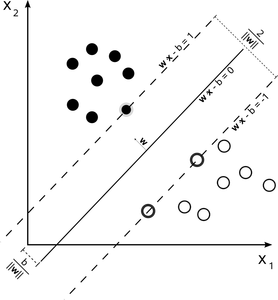
\includegraphics[width=0.75\textwidth]{imaxes/svm.png}
	\caption{Representación de un hiper plano en una SVM}
	\label{svmfigure}
\end{figure}

El hiper plano se define mediante:

\begin{equation}
\langle\overrightarrow{w}\overrightarrow{x}\rangle + b = \sum_iy_i\alpha_i\langle\overrightarrow{x_i}\overrightarrow{x}\rangle + b = 0
\end{equation}
donde \(\overrightarrow{x}\) es un vector de entrada n-dimensional e \(y_i\) es el valor de salida y \(\overrightarrow{w} = (w_1,w_2,...w_n)\) es el vector de pesos, o vector normal. Este último vector de pesos se construye mediante un conjunto de entrenamiento.

La clase de cualquier otro vector \(\overrightarrow{x_i}\) no perteneciente al conjunto de entrenamiento se puede calcular mediante la siguiente formula:

si \(\overrightarrow{w}\overrightarrow{x_i}+b \ge 0\) entonces el elemento pertenece a la clase en la que estamos interesados, si no pertenece a la otra clase.

Como vemos este caso de SVM simple, es solo válido para problemas linealmente separables, para clasificaciones más complejas es necesario mapear los datos a un espacio de mayor dimensionalidad donde se vuelvan linealmente separables utilizando funciones conocidas como funciones de \textbf{kernel}.

Para realizar una clasificación multiclase podemos proceder utilizando dos aproximaciones:

\begin{itemize}
	\item \textbf{Uno contra todos}: En esta aproximación se construye un clasificador por clase, cada uno de ellos toma una clase como positiva y el resto de clases como negativas, clasificando los elementos solo si son aceptados en dicha clase, y descartando en caso contrario.
	\item \textbf{Uno contra uno}: Se construyen clasificadores por cada par de clases y el elemento de estudio se clasifica en alguna de las dos clases pertenecientes al clasificador.
\end{itemize}

\subsubsection{Random Forest}\label{rf}

Este algoritmo desarrollado por Leo Breiman y Adele Cutler, y se trata de una combinación de árboles de decisión, tal que cada árbol depende de los valores de un vector aleatorio probado independientemente y con la misma distribución para cada uno de estos.

La idea es promediar muchos modelos ruidosos pero aproximadamente imparciales, y por lo tanto reducir la variación.

Cada árbol es construido utilizando el siguiente algoritmo:
\begin{itemize}
	\item Sea N el número de casos de prueba, M es el número de variables del clasificador.
	\item Sea m el número de variables de entrada a ser usado para determinar la decisión en un nodo dado; m debe ser mucho menor que M.
	\item Elegir un conjunto de entrenamiento para este árbol y usar el resto de los casos de prueba para estimar el error.
	\item Para cada nodo del árbol, elegir aleatoriamente m variables en las cuales basar la decisión. Calcular la mejor partición del conjunto de entrenamiento a partir de las m variables.
\end{itemize}

Para la predicción un nuevo caso es empujado hacia abajo por el árbol. Luego se le asigna la etiqueta del nodo terminal donde finaliza. Este proceso se repite por todos los árboles del modelo, y la etiqueta final será aquella con mayor cantidad de incidencias.

\subsubsection{LSTM}\label{lstmsection}

Este es el primero de los algoritmos perteneciente a la subsección de Deep Learning\footnote{Para los algoritmos que pasaremos a describir a partir de este punto se utilizaron Word Embeddings como características de los documentos en lugar de valores entre 0 y 1.}, esto quiere decir que a partir de este punto hablaremos de algoritmos que hacen uso de redes neuronales para obtener la clasificación de los documentos, comenzaremos por hacer una breve introducción a las redes neuronales para seguir describiendo el funcionamiento de las redes LSTM.

\begin{figure}[!ht]
	\centering
	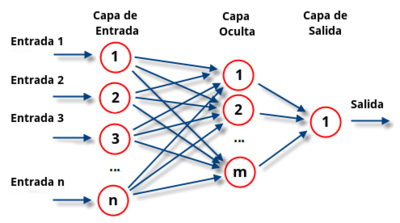
\includegraphics[width=0.75\textwidth]{imaxes/red.png}
	\caption{Representación de una red neuronal}
	\label{redneuronal}
\end{figure}

Las redes neuronales son sistemas de computación basados en las redes neuronales biológicas, que pueden ser descritas matemáticamente como \(f: X -> Y\), típicamente, están compuestas de una capa de entrada, una serie de capas ocultas y una capa de salida (ver Figura \ref{redneuronal}), en estas capas ocultas se calculan una serie de pesos \(w\) que son propagados hacia la siguiente neurona mediante la ecuación \ref{eq:8}

\begin{equation} \label{eq:8}
\mathit{p_j(t) = \sum_io_i(t)w_{ij}}
\end{equation}

Así mismo la función de una neurona \(f(x)\) es definida por una composición de otras funciones \(g_i(x)\) que pueden a su vez ser descompuestas en otras funciones. Típicamente esta función se representa como \(f(x) = K(\sum_iw_ig_i(x))\) donde \(K\) es una función de activación predefinida como una tangente parabólica, una función sigmoidal o una función softmax por ejemplo. 

Estas redes de tipo feedforward no mantienen noción de orden en el tiempo, por lo que cada input se considera solo a si mismo. Para tratar problemas del dominio del lenguaje natural necesitamos que la red tenga memoria ya que es importante el orden en el que aparecen las palabras en el documento, esto se soluciona utilizando Redes Neuronales Recurrentes en las que cada salida de una neurona es entrada de la siguiente y a su vez entrada de sí misma (ver la figura \ref{rnn}). Esta propiedad permite a estas redes tener memoria, de forma que el resultado de una salida se mantiene como información en el estado oculto de la neurona (hidden state o \(h_t\)) durante todo el proceso, esto se puede describir matemáticamente como con la ecuación \ref{eq:9}, en la que podemos ver que el estado oculto \(h_t\) recibe influencia del estado anterior \(h_{t - 1}\).

\begin{equation} \label{eq:9}
ht = \sigma(Wx-t + Uh_{t-1})
\end{equation}

Además en el entrenamiento de estas redes se utiliza un algoritmo de propagación hacia atrás (backpropagation) mediante el cual actualizamos los pesos con los resultado obtenidos en el paso de propagación de los mismos con la intención de afinar los resultados. Es posible que durante este proceso se provoquen problemas de desvanecimiento de gradiente si los pesos son muy pequeños, o de explosión de gradiente si los pesos son muy grandes, provocando divergencia en el aprendizaje.

\begin{figure}[!ht]
	\centering
	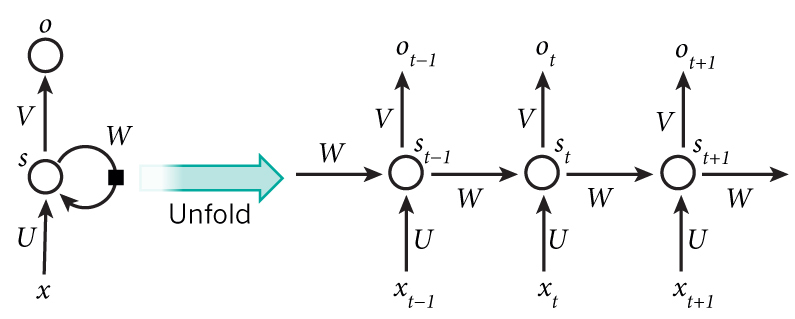
\includegraphics[width=0.75\textwidth]{imaxes/rnn.jpg}
	\caption{Representación de una red neuronal recurrente}
	\label{rnn}
\end{figure}

Estos problemas en el algoritmo de propagación hacia atrás han sido uno de los motivos detrás de la creación de las redes LSTM o Long Short-Term Memory (ver \ref{lstm}).

Las redes LSTM son un tipo de redes neuronales recurrentes propuestas en 1997 por Sepp Horchreiter y Jürgen Schmidhuber y mejoradas en el 2000 por Felix Gers junto con los autores anteriores, y han obtenido resultados record en comprensión de textos en lenguaje natural y reconocimiento de escritura manual entre otras aplicaciones. Estas redes introducen una nueva estructura llamada celda de memoria, que se compone de cuatro elementos principales:
\begin{itemize}
	\item \textbf{input gate}: permite a las señales entrantes modificar el estado de la celda de memoria.
	\item \textbf{neurona con una conexión recurrente}: permite que la celda tenga memoria
	\item \textbf{forget gate}: modula la conexión recurrente de la celda de memoria, permitiendo que recuerde u olvide los estados previos.
	\item \textbf{output gate}: permite que la celda influya sobre el resto de neuronas.
\end{itemize}

\begin{figure}[!ht]
	\centering
	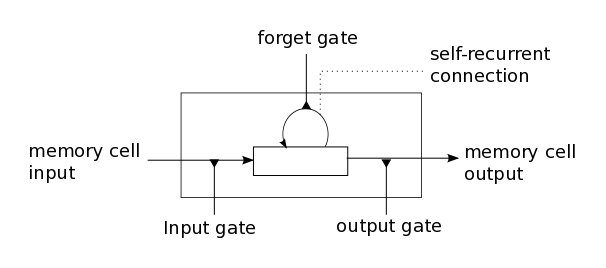
\includegraphics[width=0.75\textwidth]{imaxes/lstm.png}
	\caption{Representación de una LSTM}
	\label{lstm}
\end{figure}

El estado de una celda de memoria puede ser descrito matemáticamente como:

\begin{equation}
h_t = o_t*tanh(C_t)
\end{equation}

donde \(o_t = \sigma(W_ox_t + U_oh_{t-1} + V_oC_t + b_o)\), siendo:

\begin{equation}
C_t = i_t * \widetilde{C}_t + f_t*C_{t-1}
\end{equation}

siendo \(\widetilde{C}\) el valor candidato para el estado de la celda de memoria en el instante \(t\)

\begin{equation}
i_t = \sigma(W_ix_t + U_ih_{t-1} + b_i)
\end{equation}

\begin{equation}
\widetilde{C}_t = tanh(W_cx_t + U_ch_{t-1} + b_c)
\end{equation}

\begin{equation}
f_t = \sigma(W_fx_t + U_fh_{t-1} + b_f)
\end{equation}




\subsubsection{LSTM Doble}

En este caso nos encontramos ante el mismo algoritmo que el presentado con anterioridad, con una diferencia topológica ya que se compone de una capa de entrada, dos capas ocultas, y una capa de salida.

Las dos capas ocultas son dos LSTM, con una capa intermedia conocida como Dropout, que nos permite introducir una cierta cantidad de ruido a la red, con la intención de poder imitar el ruido existente en los problemas reales.

\subsubsection{CNN}

Este tipo de redes son ampliamente utilizadas en problemas de tratamiento de imágenes ya que se adaptan perfectamente al trabajo con pixeles, sin embargo son también muy eficaces en los problemas de lenguaje natural, además de ser más rápidas que las redes LSTM.

Como vemos en \ref{cnn} estas redes realizan una convolución utilizando ventanas de un determinado tamaño.

\begin{figure}[!ht]
	\centering
	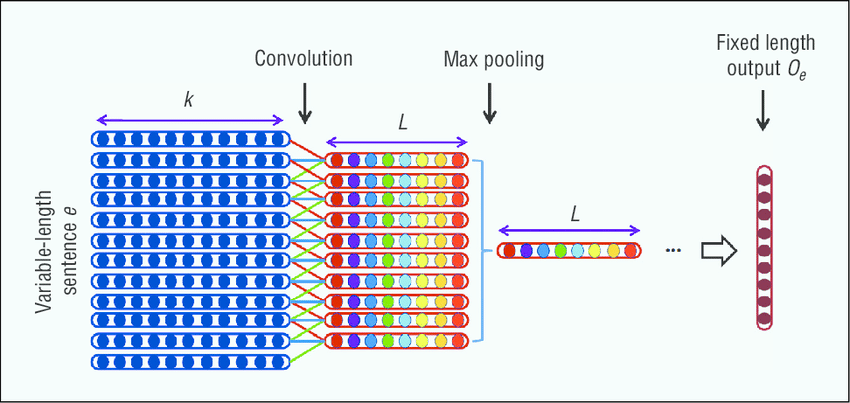
\includegraphics[width=0.75\textwidth]{imaxes/cnn1.png}
	\caption{Representación de una red CNN}
	\label{cnn}
\end{figure}

Tras la convolución utilizamos una capa de max-pool para convertir el resultado de la convolución en un gran vector de características, al igual que en el algoritmo anterior, se usa una capa de Dropout para introducir un cierto ruido en la clasificación.

Finalmente se computa la salida del clasificador mediante una capa softmax.

\subsubsection{2dCNN}

Mientras en el algoritmo CNN la ventana del filtro se componía de una sola dimensión, es decir un vector, en este caso la ventana es de dos dimensiones, de forma que la convolución actúa sobre una matriz (ver \ref{2cnn}).

\begin{figure}[!ht]
	\centering
	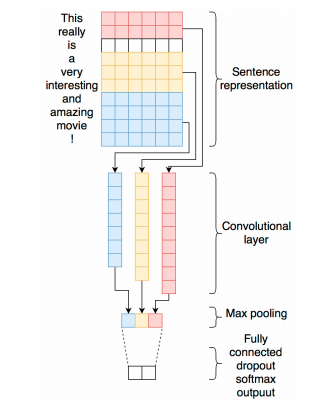
\includegraphics[width=0.75\textwidth]{imaxes/cnn.png}
	\caption{Representación de una red CNN}
	\label{2cnn}
\end{figure}

Esta versión del algoritmo nos permite tratar a la vez grupos de palabras y no solo ciertas partes del word embedding, de esta forma el algoritmo es capaz de tratar n-gramas de forma natural.

\subsubsection{2dCNN + LSTM}

Este es el primer caso en el que se experimenta con una composición de algoritmos, es decir, se usa un algoritmo híbrido, de forma que la red neuronal se compone de una capa de convolución de dos dimensiones que convierte varias palabras en un vector de características que se utilizará como entrada de las celdas de memoria de la capa LSTM que la sigue. De esta forma queremos combinar las bondades del tratamiento de n-gramas de las redes convolucionales con la capacidad de memoria de las redes LSTM.

\subsubsection{Bidirectional LSTM}\label{bidi}

Este tipo de topología LSTM se compone de dos redes LSTM individuales, con una característica importante: la primera capa recibe los datos en su estado normal aprendiendo de atrás hacia adelante, y la segunda recibe los datos de forma invertida, de forma que puede aprender el efecto que tienen los datos en el ``pasado''.

Los resultados de estas dos redes se combinan en una capa de fusionado con una estrategia multiplicativa.

\section{Servicio web}


\subsection{Visualizar comentarios}

Se expone un endpoint, disponible mediante un método GET de HTTP que recibirá como parámetro un id de articulo.

Este endpoint buscará en la base de datos los comentarios relacionados con el artículo y lo devolverá al cliente mediante un array de objetos.

\subsection{Añadir comentarios}

Se expone un endpoint del servicio, que recibirá un objeto comentario y un id de articulo mediante un método PUT. Este método guardará el contenido del comentario en la base de datos relacionándolo con el artículo mediante una clave foránea.

\subsection{Editar comentarios}

El cliente enviará una petición POST a un endpoint del servicio, enviando el nuevo contenido del comentario y el identificador del comentario a editar.

\subsection{Borrar comentarios}

Mediante una petición DELETE que incluya un identificador de comentario, el servicio realizará un borrado del comentario en la base de datos.

 
\chapter{Resultados}

\lettrine{E}{n} este capítulo analizaremos los resultados obtenidos en los modelos estudiados, realizando en todos ellos una división de los datos de entrenamiento mediante K-Folds, que nos permite comparar los modelos según precisión media.

\section{Corpus de datos}\label{corpus}

\subsection{Corpus TASS}
Se trata de un corpus ofrecido por el TASS \footnote{http://www.sepln.org/workshops/tass/2016/tass2016.php}, taller que se centra en las tareas de análisis de sentimientos y de reputación para el idioma español, organizado como evento satélite en la conferencia anual de la SEPLN (Sociedad Española para el Procesamiento del Lenguaje Natural).

Proponen dos tipos de clasificaciones: una basada en un sistema de 6 clases (Positivo +, Positivo, Neutro, Negativo, Negativo +, None) y otra en 4 clases (Negativo, Neutro, Positivo, None).

Para ello ofrecen un conjunto de 6800 tweets para entrenamiento, que vienen acompañados de una polaridad supervisada que se encontrará dentro del rango de 6 clases anteriormente citado.

\begin{figure}[!ht]
	\centering
	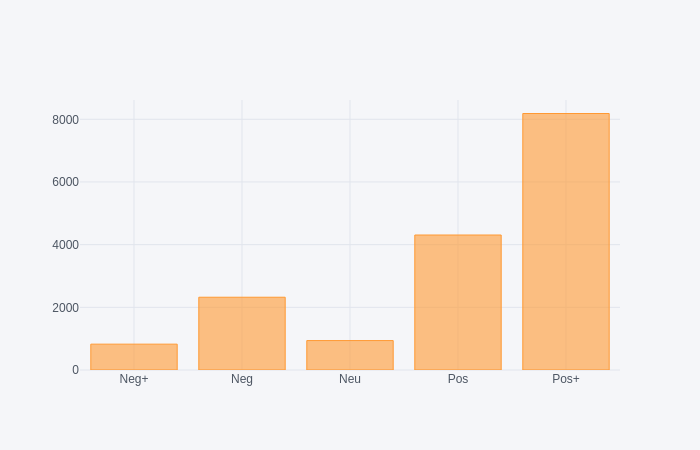
\includegraphics[width=0.75\textwidth]{imaxes/distTass.png}
	\caption{Distribución de la polarización.}
	\label{dist_tass}
\end{figure}

\begin{figure}[!ht]
	\centering
	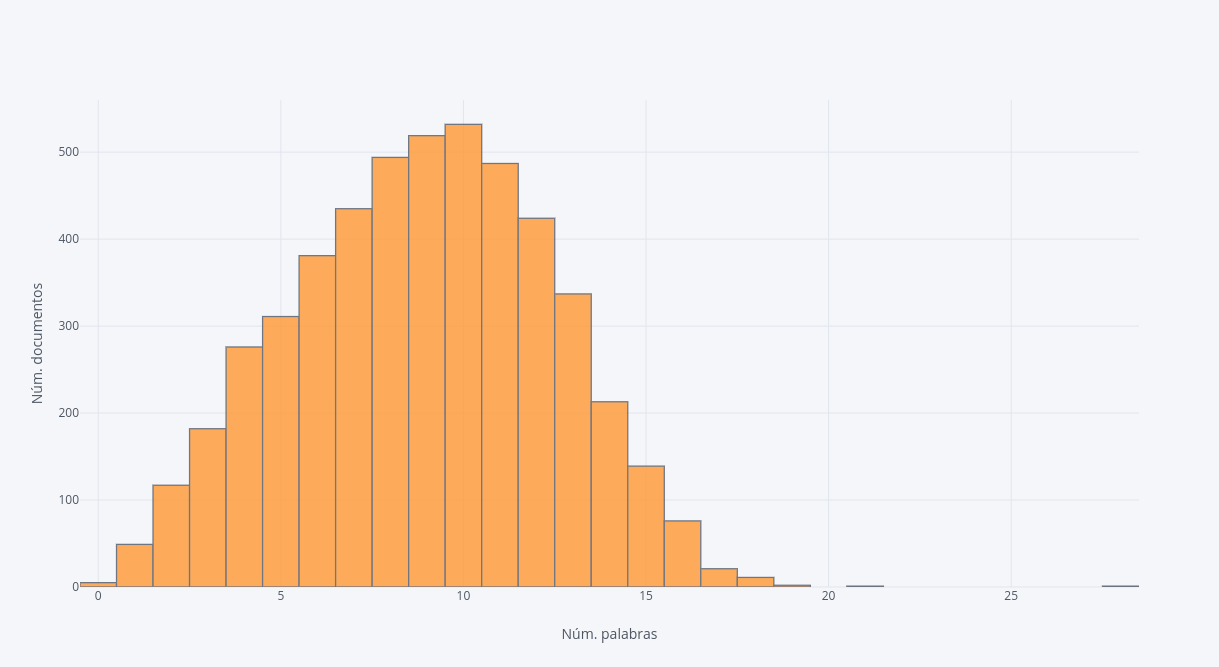
\includegraphics[width=1\textwidth]{imaxes/distTokensTass.png}
	\caption{Histograma de número de palabras por documento.}
	\label{dist_tokes_tass}
\end{figure}

En la figura \ref{dist_tass} vemos una distribución con tendencia hacia los extremos, sobre todo a las polaridades positivas, mientras que la figura \ref{dist_tokes_tass} nos muestra que la mayoría de los documentos contienen tan solo 10 o menos palabras, alcanzando un máximo de 28.

Hemos traducido un lexicón de palabras polarizadas del inglés para cruzarlos con los tweets de la colección y comprobar la distribución de las palabras en los mismos, obteniendo los siguientes resultados:

\begin{figure}[H]
	\centering
	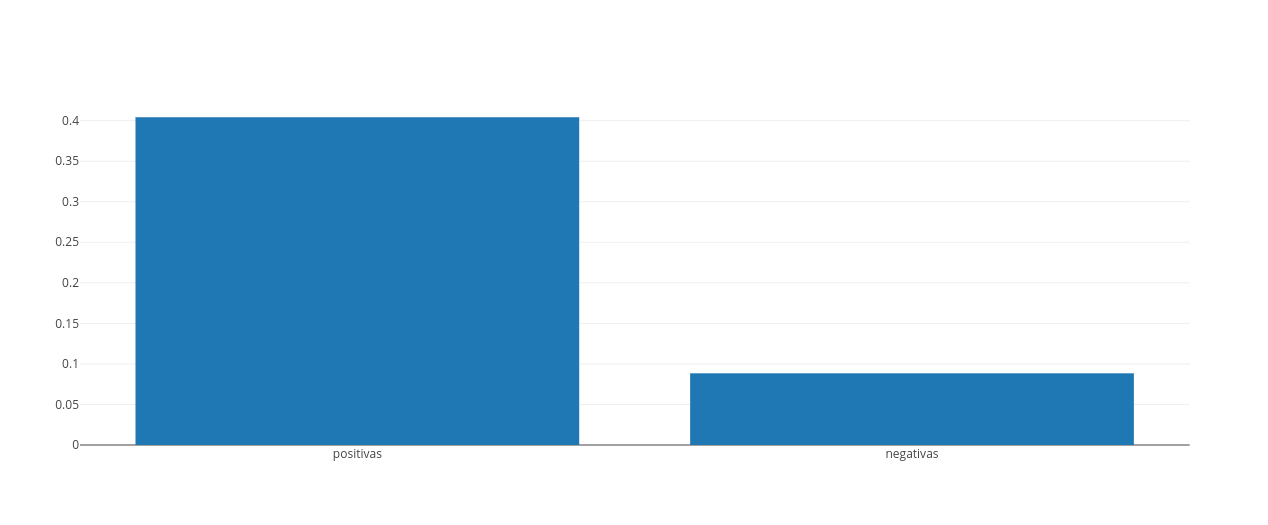
\includegraphics[width=0.75\textwidth]{imaxes/dist_pos_neg.png}
	\caption{Distribución de las palabras polarizadas en tweets positivos}
	\label{dist_pos}
\end{figure}

Como se ve en la figura \ref{dist_pos} los tweets positivos presentan un cantidad notablemente mayor de palabras positivas, por lo que podemos deducir, que la clasificación de estos tweets en su clase debería ser sencilla, si somos capaces de eliminar correctamente todas las palabras que puedan aportar ruido innecesario al modelo.

\begin{figure}[H]
	\centering
	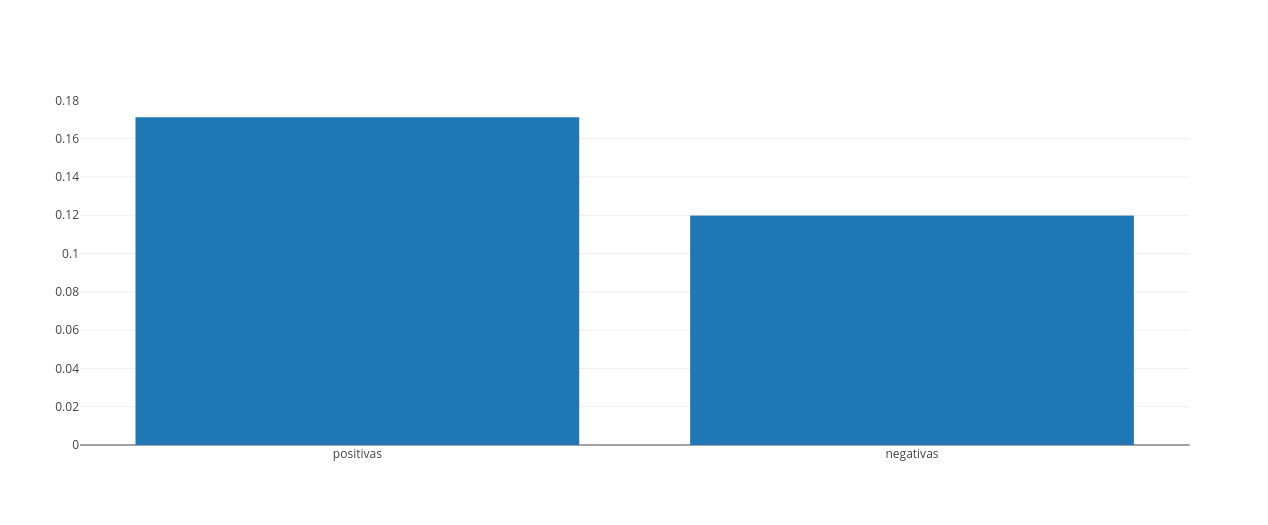
\includegraphics[width=0.75\textwidth]{imaxes/dist_pos_neg_neg.png}
	\caption{Distribución de las palabras polarizadas en tweets negativos}
	\label{dist_neg}
\end{figure}

En el caso de los tweets negativos la gráfica \ref{dist_neg} podemos observar que está más compensada, por lo que será más complicado para el modelo discernir la clase de estos tweets

\begin{figure}[!ht]
	\centering
	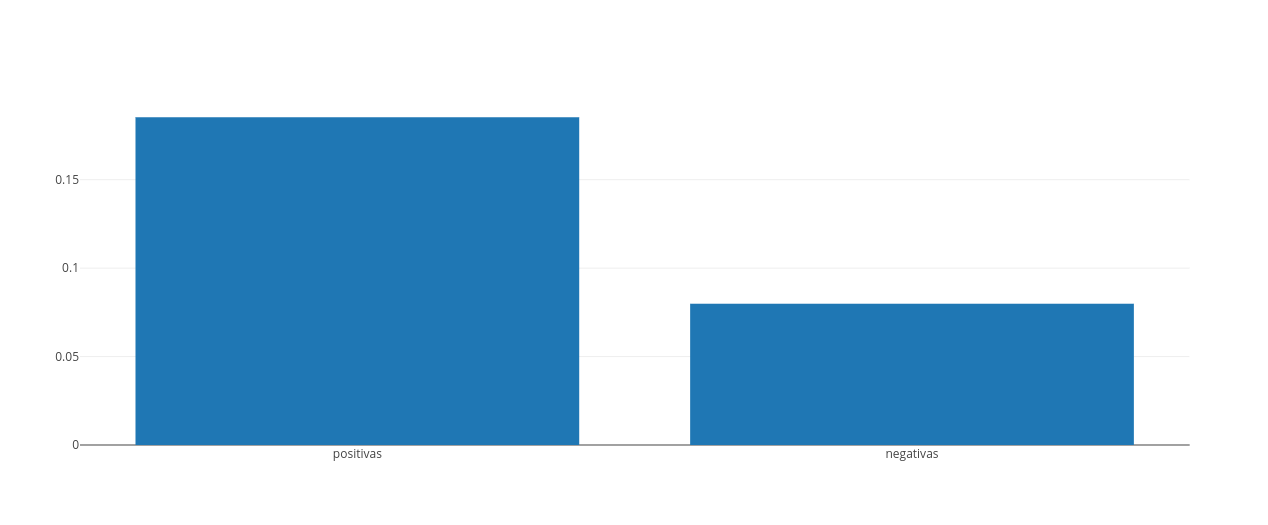
\includegraphics[width=0.75\textwidth]{imaxes/dist_pos_neg_neut.png}
	\caption{Distribución de las palabras polarizadas en tweets neutros}
	\label{dist_neut}
\end{figure}

Para los tweets con clase neutral, se encuentran más palabras positivas que negativas, con lo que es muy probable que estos tweets acaben clasificados en una clase positiva.

Dado este análisis podemos deducir que el modelo de clasificación tendrá facilidad al clasificar los tweets positivos, pero dificultades al clasificar el resto. Esta tendencia del lenguaje a mostrar positividad ya ha sido demostrada por diversos estudios como los propuestos por Kloumann, Isabel M et al. \cite{PoeEL} y Dodds, Peter Sheridan et al. \cite{HulPB}.

\subsection{Corpus Cine}

Ya que en el momento actual no tenemos conocimiento de como van a ser los textos reales del dominio de la aplicación necesitamos probar los modelos contra textos más extensos y escritos de una forma más formal.

Se trata de un corpus descargado de la página MuchoCine.com para el trabajo, con la intención de disponer de un conjunto de documentos más extenso, tanto en número de documentos como en cantidad de palabras por documento (ver fig. \ref{dist_tokes_pelis}).

Estos documentos están clasificados con un sistema de cinco estrellas que se puede traducir a la clasificación realizada en nuestro sistema de la siguiente forma:

\begin{itemize}
	\item 5 estrellas: Positivo+.
	\item 4 estrellas: Positivo.
	\item 3 estrellas: Neutro.
	\item 2 estrellas: Negativo.
	\item 1 estrella: Negativo+.
\end{itemize}

Con esto podremos comprobar el funcionamiento de los modelos en un dominio distinto al del conjunto de entrenamiento, y comprobar si son aptos para desplegar en producción.

\begin{figure}[!ht]
	\centering
	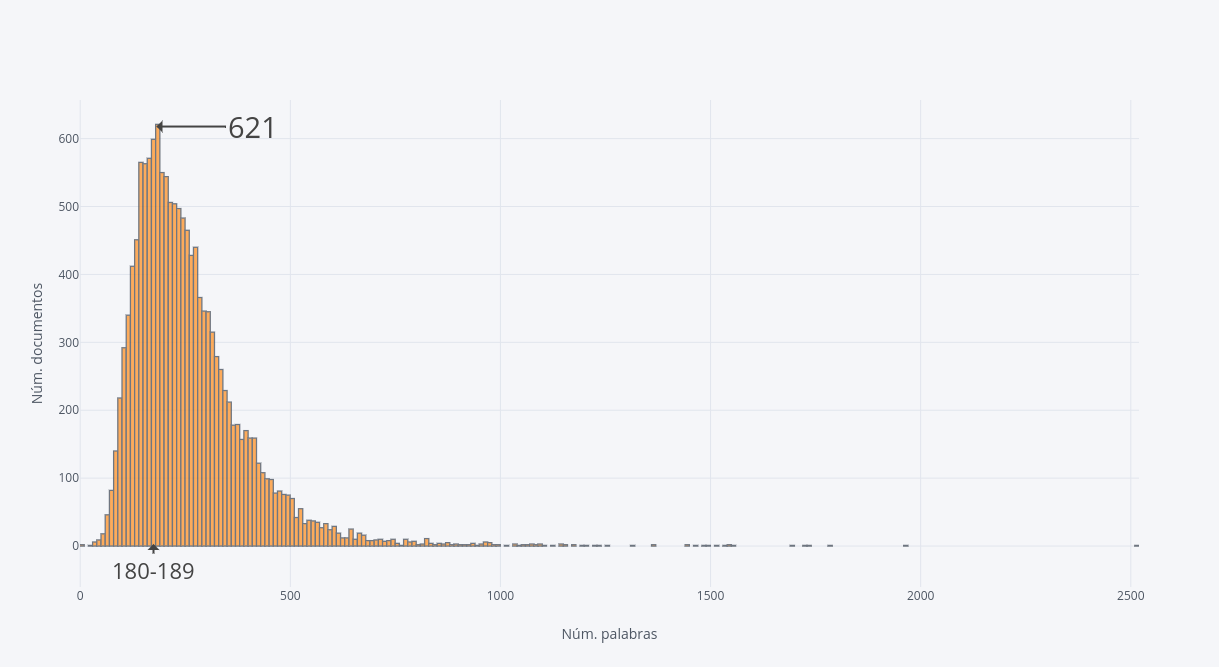
\includegraphics[width=1\textwidth]{imaxes/distTokensCine.png}
	\caption{Histograma de número de palabras por documento.}
	\label{dist_tokes_pelis}
\end{figure}

Está compuesto por un total de 5000 documentos con un alto número de oraciones por documento en comparación con el corpus TASS.

\begin{figure}[!ht]
	\centering
	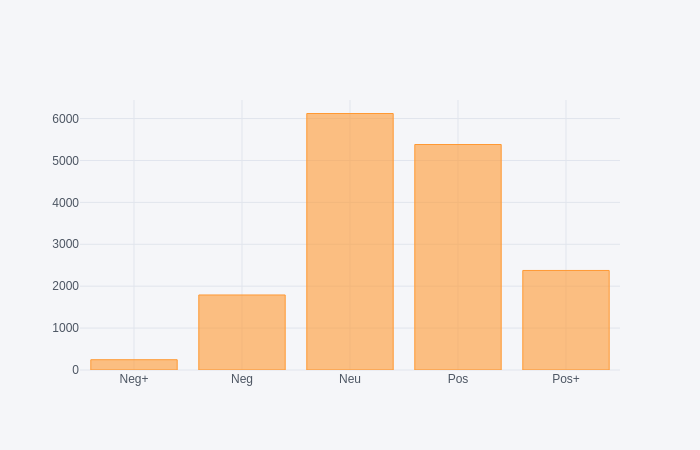
\includegraphics[width=0.75\textwidth]{imaxes/distCine.png}
	\caption{Distribución de la polarización.}
	\label{dist_pos_pelis}
\end{figure}

En este caso los usuarios de la red tienen tendencia a realizar críticas con valoraciones medias, encontrando muy pocos casos en los extremos.


\section{Machine learning}\label{sect:ML}

En las siguientes secciones comprobaremos el funcionamiento de los modelos para la clasificación de documentos del mismo dominio (TASS) y de distinto dominio (Cine).

Para establecer una línea base sobre la que probar  nuevos modelos o mejoras se ha realizado un entrenamiento con los parámetros por defecto de los modelos explicados en la sección \ref{alg}: MNB, LR, SVM, RF.


\subsection{Línea base}

\subsubsection{2 clases}

\begin{table}[H]
	\centering
	\begin{tabular}{|l|cccc|cccc|}
		\hline
		& \multicolumn{4}{c|}{TASS} & \multicolumn{4}{c|}{CINE} \\
		\cline{2-9}
		&    acc &     f1 &    mse &  recall & acc &     f1 &    mse &  recall \\
		\hline
		lr      &  77.17 &  81.07 &  22.83 &   77.54 &  51.48 &  33.48 &  48.52 &   79.37 \\
		ls      &  77.29 &  81.02 &  22.71 &   78.01 &  49.08 &  26.58 &  50.92 &   78.07 \\
		mb      &  79.97 &  \textbf{82.32} &  20.03 &   83.78 &  62.63 &  \textbf{63.90} &  37.37 &   72.04 \\
		rf      &  73.92 &  78.60 &  26.08 &   74.54 &  51.88 &  48.44 &  48.12 &   63.21 \\
		\hline
	\end{tabular}
	\caption{Resultados en \% entrenamiento para línea base.}
	\label{result-línea-base}
\end{table}

El modelo con mejores resultados es MNB, con un resultado de f1 de 82.32\% para el corpus TASS y un 63.90\% para el corpus de críticas de cine.


\subsubsection{3 clases}

\begin{table}[H]
	\centering
	\begin{tabular}{|l|cccc|cccc|}
		\hline
		& \multicolumn{4}{c|}{TASS} & \multicolumn{4}{c|}{CINE} \\
		\cline{2-9}
		&    acc &     f1 &    mse &  recall & acc &     f1 &    mse &  recall \\
		\hline
		lr      &  72.31 &  72.31 &   93.62 &   72.31 &  31.19 &  31.19 &  150.51 &   31.19 \\
		ls      &  72.40 &  72.40 &   93.34 &   72.40 &  28.63 &  28.63 &  162.97 &   28.63 \\
		mb      &  73.19 &  \textbf{73.19} &   81.34 &   73.19 &  37.35 &  \textbf{37.35} &  128.21 &   37.35 \\
		rf      &  68.05 &  68.05 &  110.27 &   68.05 &  32.78 &  32.78 &  137.66 &   32.78 \\
		\hline
	\end{tabular}
	\caption{Resultados en \% entrenamiento para línea base de 3 clases.}
	\label{result-línea-base-3-clases}
\end{table}

Al igual que en el caso de la clasificación binaria, el modelo con mejores resultados es el de Bayes con un 73.19\% para el TASS y un 37.35\% para las críticas de cine.

\subsubsection{5 clases}

\begin{table}[H]
	\centering
	\begin{tabular}{|l|cccc|cccc|}
		\hline
		& \multicolumn{4}{c|}{TASS} & \multicolumn{4}{c|}{CINE} \\
		\cline{2-9}
		&    acc &     f1 &    mse &  recall & acc &     f1 &    mse &  recall \\
		\hline
		lr      &  48.33 &  48.33 &  225.23 &   48.33 &  18.50 &  \textbf{18.50 }&  277.25 &   18.50 \\
		ls      &  48.09 &  48.09 &  240.97 &   48.09 &  16.09 &  16.09 &  307.73 &   16.09 \\
		mb      &  50.73 &  \textbf{50.73} &  200.21 &   50.73 &  16.47 &  16.47 &  302.59 &   16.47 \\
		rf      &  43.53 &  43.53 &  243.98 &   43.53 &  17.92 &  17.92 &  298.46 &   17.92 \\
		\hline
	\end{tabular}
	\caption{Resultados en \% entrenamiento para línea base de 5 clases.}
	\label{result-línea-base-5-clases}
\end{table}

En este caso las clasificaciones han bajado notablemente el resultado de la medida f1, obteniendo un 50.73\% para Bayes, pero en el caso del corpus de Cine las clasificaciones se encuentran por debajo de la aleatoriedad (20\% por ser 5 clases).

En el material anexo (sección \ref{analisis_bl_5}) se muestra un estudio sobre las causas de esta problemática.

\subsection{Experimentos de mejora Machine Learning}

Los experimentos han comenzado por un intento de mejora de los algoritmos de machine learning.

Como se menciona en \ref{sect:ML} para el establecimiento de la línea base se han utilizado los parámetros por defecto de los algoritmos. Para intentar encontrar una mejor combinación se ha realizado una validación cruzada de los siguientes parámetros:

\begin{itemize}
	\item Preprocesado de la negación (Verdadero o falso).
	\item Eliminación de carácteres repetido (Verdadero o falso).
	\item Rango de n-gramas (1 o 2).
	\item Tokenización o Stemming.
	\item Máximo número de iteraciones para SVM (1000, 2000, 1500).
	\item Máximo número de iteraciones para LR (100, 200, 500).
	\item Modificación del parámetro alpha para MB (1.0, 0.5 o 1.5).
	\item Número de estimadores para RF (10 o 100).
\end{itemize}

Además se han repetido el proceso utilizando como preprocesador CountVectorizer y TFIDF.



\subsubsection{2 clases}

\begin{table}[H]
	\centering
	\begin{tabular}{|l|cccc|cccc|}
		\hline
		& \multicolumn{4}{c|}{CountVectorizer} & \multicolumn{4}{c|}{TF-IDF} \\
		\cline{2-9}
		&    acc &     f1 &    mse &  recall & acc &     f1 &    mse &  recall \\
		\hline
		lr      &  79.18 &  82.52 &  20.82 &   79.94 &  77.96 &  81.98 &  22.04 &   77.56 \\
		ls      &  78.24 &  81.70 &  21.76 &   79.24 &  79.97 &  82.87 &  20.03 &   81.63 \\
		mb      &  80.61 &  \textbf{82.90} &  19.39 &   84.20 &  79.18 &  \textbf{83.09} &  20.82 &   78.07 \\
		rf      &  75.14 &  78.85 &  24.86 &   77.30 &  73.89 &  78.03 &  26.11 &   75.75 \\
		\hline
	\end{tabular}
	\caption{Medias en \% entrenamiento para gridsearch con 2 clases.}
	\label{result-cv-kf}
\end{table}

En la tabla \ref{result-cv-kf} vemos que hemos conseguido mejorar la puntuación de todos los algoritmos. Cabe destacar el resultado del modelo de Bayes con un resultado cercano al 83\% en cualquiera de los métodos de selección de características.

\subsubsection{3 clases}

\begin{table}[H]
	\centering
	\begin{tabular}{|l|cccc|cccc|}
		\hline
		& \multicolumn{4}{c|}{CountVectorizer} & \multicolumn{4}{c|}{TF-IDF} \\
		\cline{2-9}
		&    acc &     f1 &    mse &  recall & acc &     f1 &    mse &  recall \\
		\hline
		lr      &  68.88 &  68.88 &  106.81 &   68.88 &  73.68 &  73.68 &   88.24 &   73.68 \\
		ls      &  67.84 &  67.84 &  111.58 &   67.84 &  74.95 &  \textbf{74.95} &   83.13 &   74.95 \\
		mb      &  70.12 &  \textbf{70.12} &  101.82 &   70.12 &  74.68 &  74.68 &   84.22 &   74.68 \\
		rf      &  66.63 &  66.63 &  111.79 &   66.63&  68.81 &  68.81 &  106.78 &   68.81 \\
		\hline
	\end{tabular}
	\caption{Medias en \% entrenamiento para gridsearch con 3 clases.}
	\label{result-cv-kf-3-clases}
\end{table}

En la tabla \ref{result-cv-kf-3-clases} vemos que el algoritmo tf-idf se comporta mejor ante la presencia de elementos con polaridad neutra. En este caso el modelo SVM es el de mayor puntuación.

\subsubsection{5 clases}

\begin{table}[H]
	\centering
	\begin{tabular}{|l|cccc|cccc|}
		\hline
		& \multicolumn{4}{c|}{CountVectorizer} & \multicolumn{4}{c|}{TF-IDF} \\
		\cline{2-9}
		&    acc &     f1 &    mse &  recall & acc &     f1 &    mse &  recall \\
		\hline
		lr      &  45.29 &  45.29 &  250.52 &   45.29 &  50.64 &  50.64 &  214.38 &   50.64 \\
		ls      &  44.68 &  44.68 &  284.19 &   44.68 &  50.70 &  \textbf{50.70} &  203.83 &   50.70 \\
		mb      &  46.41 &  \textbf{46.41} &  246.11 &   46.41 &  48.97 &  48.97 &  228.30 &   48.97 \\
		rf      &  39.57 &  39.57 &  278.27 &   39.57 &  45.08 &  45.08 &  241.49 &   45.08 \\
		\hline
	\end{tabular}
	\caption{Medias en \% entrenamiento para gridsearch con 5 clases.}
	\label{result-cv-kf-5-clases}
\end{table}

Como se muestra en la tabla \ref{result-cv-kf-5-clases} el algoritmo tf-idf es el que mayores puntuaciones obtiene, destacando el modelo SVM con una puntuación de 50.70\%.


\subsubsection{Conclusiones}

Si comparamos los dos métodos de preprocesado de textos que hemos utilizado vemos que el Tf-idf es el que mejores resultados obtiene para todos los casos de clasificación.

En cuanto a los mejores parámetros, hemos obtenido valores dispares en cuanto al parámetro estudiado de cada algoritmo, sin embargo en todos los casos se establecido como necesario el tratamiento de la negación, el uso de Stemming y el preprocesado de letras repetidas. En cuanto al rango de n-gramas en la mayoría de los casos se ha obtenido un valor de 1.

En cuanto a los modelos vemos que Bayes es el que mejor funciona para el CountVectorizer sin embargo en el otro caso es el modelo SVM el que mayor puntuación obtiene.

Con esto podemos deducir que deberíamos escoger Tf-idf como selector de características y el modelo SVM para realizar las clasificaciones.

En el material anexo se incluyen también resultados de adaptación al dominio para los modelos optimizados por grid search. Si comparamos los resultados de los clasificadores en el conjunto de test (tablas \ref{result-cv-test}, \ref{result-cv-test-3-clases} y \ref{result-cv-test-5-clases}) con los resultados en el dominio de críticas de cine (tablas \ref{result-cv-test-cine}, \ref{result-cv-test-3-clases-cine} y \ref{result-cv-test-5-clases-cine}) vemos que los modelos son tolerantes a la aparición de nuevos datos del mismo dominio pero su rendimiento baja notablemente en el otro caso. Esto se debe a que el algoritmo de selección de características está limitado a los elementos encontrados en el primer dominio y el resto de elementos del segundo dominio no serán tenidos en cuenta, provocando pérdida de información.


\section{Deep Learning}

En esta sección se mostrarán los resultados de los entrenamientos de modelos de Deep Learning.

Para estos casos se ha realizado una selección de parámetros manual sobre un modelo LSTM base, y posteriormente se han ejecutado el resto de algoritmos en la sección \ref{alg}. 

Todos los entrenamientos realizan 30 iteraciones (epochs).

\subsection{Selección de parámetros}

En esta sección mostraremos un ejemplo ilustrativo de como se ha iterado para la selección de parámetros de un modelo LSTM sobre el corpus TASS.

Este proceso se debe repetir para todas las distribuciones de clases y para todos los modelos.

\subsubsection{Base}

Este modelo se ha configurado con 64 neuronas en la capa oculta, y una activación RELU (fig. \ref{relu}) que limita las salidas de la capa a un valor entre 0 e infinito.

\begin{figure}[!ht]
	\centering
	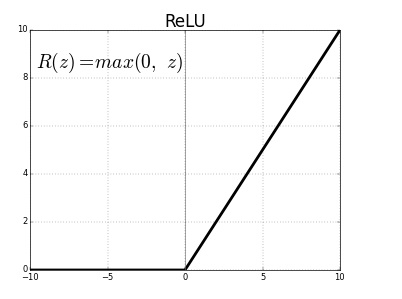
\includegraphics[width=0.75\textwidth]{imaxes/relu.jpg}
	\caption{Función de activación RELU}
	\label{relu}
\end{figure}

La gráfica \ref{evo_lstm_base} muestra la evolución de la pérdida en los conjuntos de entrenamiento y validación durante las 30 iteraciones del entrenamiento. Se han eliminado los valores con picos muy altos para facilitar la lectura.
Podemos ver que hacia el final del entrenamiento los valores de validación empiezan a divergir de los valores del conjunto de entrenamiento, esto es indicativo de que se comienza a producir un sobre entrenamiento.

\begin{figure}[H]
	\centering
	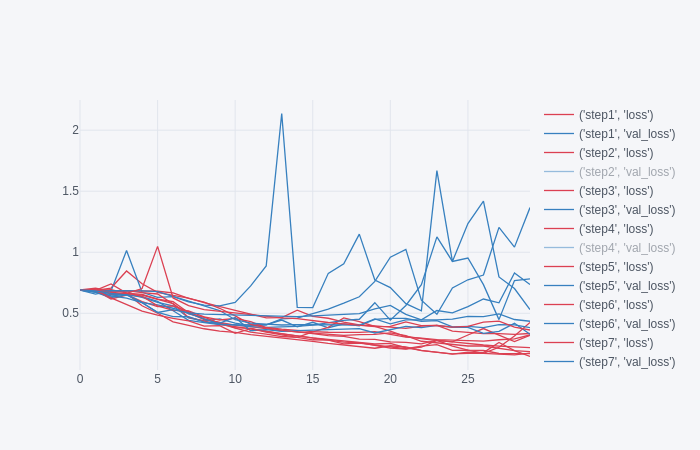
\includegraphics[width=0.75\textwidth]{imaxes/baselstm.png}
	\caption{Evolución entrenamiento modelo LSTM}
	\label{evo_lstm_base}
\end{figure}


El sobre entrenamiento generalmente es síntoma de un modelo excesivamente complejo y por lo tanto provoca un alto nivel de varianza ajustándose en exceso a los casos de entrenamiento. Para solucionar esto se ha probado un modelo más simple de 10 neuronas.

La evolución del modelo simplificado (\ref{simple}) muestra menos rasgos de sobre entrenamiento manteniendo más tiempo la tendencia a reducir la pérdida en el conjunto de validación.

\begin{figure}[H]
	\centering
	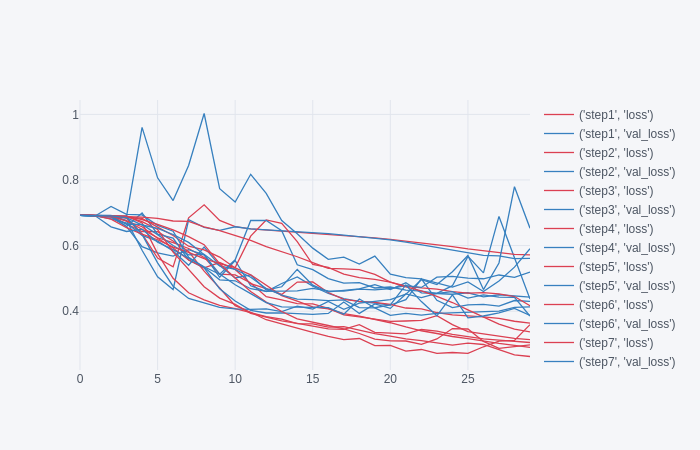
\includegraphics[width=0.75\textwidth]{imaxes/simple.png}
	\caption{Evolución entrenamiento modelo LSTM simplificado}
	\label{simple}
\end{figure}

Dado que la tendencia de este modelo es buena se han realizado pruebas configurando otros parámetros, como:

\begin{itemize}
	\item Dropout: Se introduce ruido sintético al modelo, apagando de forma aleatoria las neuronas durante el entrenamiento.
	\item Inicialización de pesos: Se cambia la inicialización de los pesos de las neuronas de la capa oculta, utilizando un tipo de inicialización conocida como Xavier initilization \cite{Glorot} o glorot normal, la cual asigna pesos de una distribución normal truncada centrada en el 0.
	\item Normalización de batch: Se normaliza la salida de la anterior capa de activación restando la media del batch y dividiendo por desviación típica. Con esto se consiguen entrenamientos más rápidos y menor varianza entre los resultados.
\end{itemize}

En la figura \ref{dropout02} vemos como han desaparecido los picos de las primeras iteraciones y parece que la evolución del entrenamiento es más adecuada, de forma que el modelo puede ser apto para seguir seleccionando mejores configuraciones.

\begin{figure}[H]
	\centering
	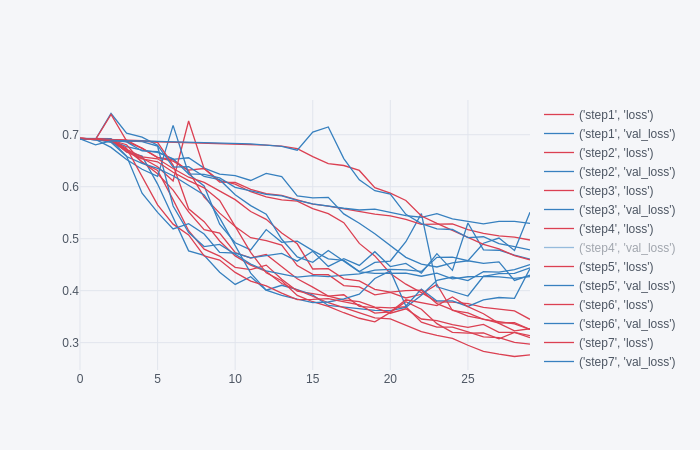
\includegraphics[width=0.75\textwidth]{imaxes/dropout0_2.png}
	\caption{Dropout con valor 0.2}
	\label{dropout02}
\end{figure}

En el siguiente experimento (fig. \ref{glorot}) se aprecia se aprecia mayor uniformidad en la evolución si despreciamos los picos, que pueden ser debidos a una distribución poco favorable para este modelo. Sin embargo cuando aplicamos además la normalización de batch, aunque conseguimos eliminar los picos, vemos que se produce sobre entrenamiento en las primeras etapas.


\begin{figure}[H]
	\centering
	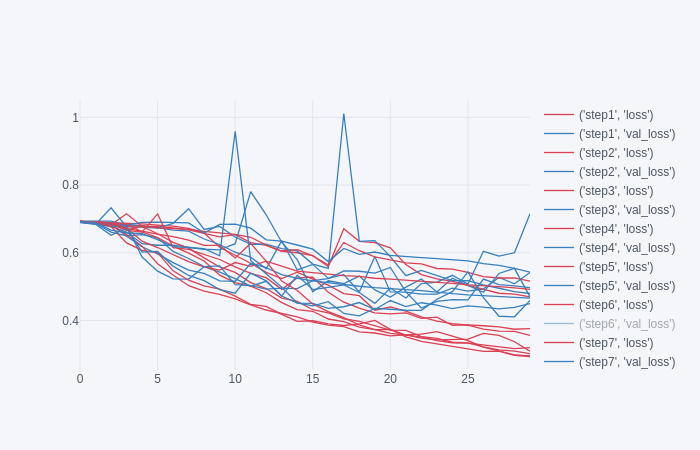
\includegraphics[width=0.75\textwidth]{imaxes/glorot.png}
	\caption{Inicialización Glorot más Dropout}
	\label{glorot}
\end{figure}

\begin{figure}[H]
	\centering
	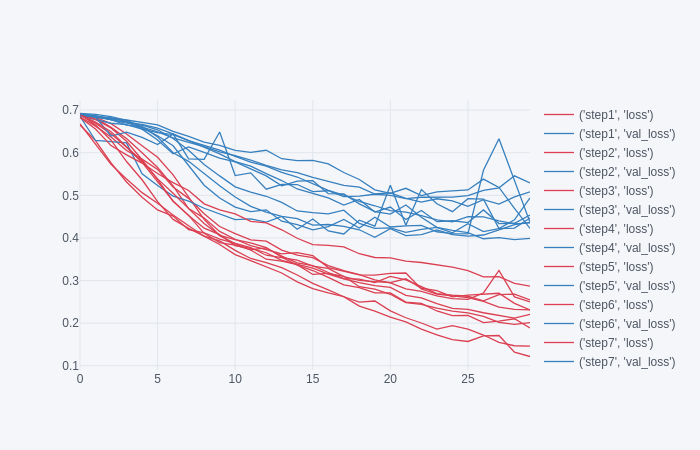
\includegraphics[width=0.75\textwidth]{imaxes/glorot_bn.png}
	\caption{Inicialización Glorot, dropout y normalización de batch}
	\label{glorotbn}
\end{figure}

Por lo tanto deberíamos quedarnos con el modelo con Dropout para seguir investigando ya que los otros parámetros no han dado resultados satisfactorios.



\subsection{2 clases}

\begin{table}[H]
	\centering
	\begin{tabular}{|l|cccc|cccc|}
		\hline
		& \multicolumn{4}{c|}{TASS} & \multicolumn{4}{c|}{CINE} \\
		\cline{2-9}
		&    acc &     f1 &    mse &  recall & acc &     f1 &    mse &  recall \\
		\hline
		base          &  80.21 &  80.34 &  19.79 &   94.84 &  49.54 &  31.90 &  50.46 &   71.72 \\
		simpler       &  81.42 &  83.21 &  18.58 &   87.47 &  56.46 &  60.81 &  43.54 &   63.16 \\
		dropout  &  81.84 &  84.24 &  18.16 &   84.86 &  58.92 &  69.71 &  41.08 &   60.61\\
		batch norm    &  82.27 &  85.12 &  17.73 &   82.95 &  57.80 &  \textbf{72.05} &  42.20 &   58.26\\
		glorot        &  81.56 &  84.97 &  18.44 &   80.59  &  58.26 &  66.35 &  41.74 &   61.95\\
		glorot\_wo\_bn  &  83.97 &  \textbf{85.80} &  16.03 &   88.24 &  56.58 &  60.20 &  43.42 &   63.79\\
		double        &  81.70 &  82.73 &  18.30 &   91.42 &  52.38 &  43.70 &  47.62 &   68.55\\
		conv          &  78.94 &  79.01 &  21.06 &   93.63 &  55.60 &  55.83 &  44.40 &   65.41\\
		conv2d        &  81.42 &  84.93 &  18.58 &   80.22 &  56.14 &  63.19 &  43.86 &   61.18\\
		bidirectional &  81.06 &  82.49 &  18.94 &   88.97 &  52.30 &  46.34 &  47.70 &   65.86 \\
		\hline
	\end{tabular}
	\caption{Resultados sobre el conjunto de test.}
	\label{test-dl-2-clases}
\end{table}

La tabla \ref{test-dl-2-clases} nos muestra el resultado de la clasificación del conjunto de test con los  modelos entrenados sobre todo el conjunto de entrenamiento. 

Vemos que los modelos con mejores resultados son los expuestos en la sección anterior, debido a que la optimización de parámetros ha permitido reducir la variación entre los resultados de las distintas particiones y por lo tanto son más robustos ante distintas distribuciones.

Cabe destacar el modelo con inicialización Glorot con 85.80\% en la medida f1, superando el 83.09\% obtenido como máximo en los modelos de Machine Learning.


\subsection{3 clases}

\begin{table}[H]
	\centering
	\begin{tabular}{|l|cccc|cccc|}
		\hline
		& \multicolumn{4}{c|}{TASS} & \multicolumn{4}{c|}{CINE} \\
		\cline{2-9}
		&    acc &     f1 &    mse &  recall & acc &     f1 &    mse &  recall \\
		\hline
		base          &  74.25 &  74.25 &  80.64 &   74.25 &  34.02 &  34.02 &  141.52 &   34.02\\
		simpler       &  75.25 &  75.25 &  76.65 &   75.25 &  33.58 &  33.58 &  143.10 &   33.58\\
		dropout  &  75.32 &  75.32 &  76.38 &   75.32 &  30.90 &  30.90 &  154.00 &   30.90\\
		batch norm    &  77.18 &  \textbf{77.18} &  68.93 &   77.18 &  34.24 &  34.24 &  140.64 &   34.24\\
		glorot        &  76.58 &  76.58 &  71.32 &   76.58 &  22.78 &  22.78 &  186.48 &   22.78 \\
		glorot\_wo\_bn  &  74.18 &  74.18 &  80.90 &   74.18 &  35.08 &  35.08 &  137.46 &   35.08\\
		double        &  74.12 &  74.12 &  81.17 &   74.12 &  31.48 &  31.48 &  151.96 &   31.48\\
		conv          &  73.25 &  73.25 &  77.64 &   73.25 &  35.74 &  \textbf{35.74} &  133.32 &   35.74\\
		conv2d        &  73.52 &  73.52 &  76.78 &   73.52 &  29.40 &  29.40 &  160.06 &   29.40\\
		bidirectional &  75.58 &  75.58 &  71.52 &   75.58 &  34.92 &  34.92 &  137.86 &   34.92\\
		\hline
	\end{tabular}
	\caption{Resultados sobre el conjunto de test.}
	\label{test-dl-3-clases}
\end{table}

En este experimento la mayor puntuación obtenida ha sido de 77.18\% por un modelo LSTM con normalización de batch, superando el 73\% obtenido con Machine Learning. 

La introducción de elementos neutros en el conjunto de datos produce picos de pérdida muy altos en los modelos, los cuales son suavizados gracias a la normalización de batch.

\begin{figure}[H]
	\centering
	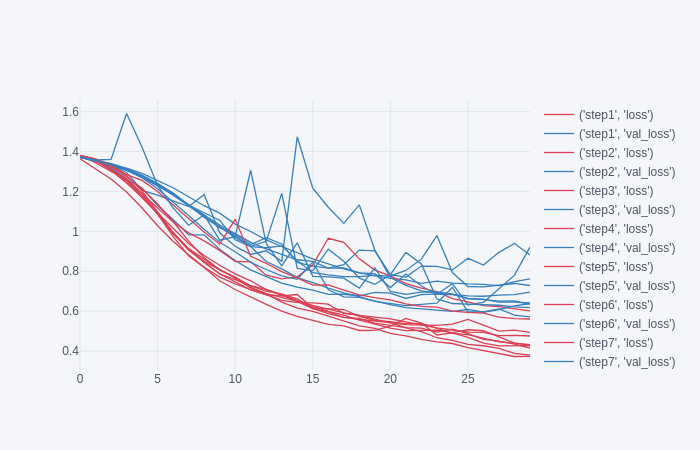
\includegraphics[width=0.75\textwidth]{imaxes/bn-3.png}
	\caption{Evolución modelo LSTM con normalización de batch.}
	\label{bn-3}
\end{figure}

\begin{figure}[H]
	\centering
	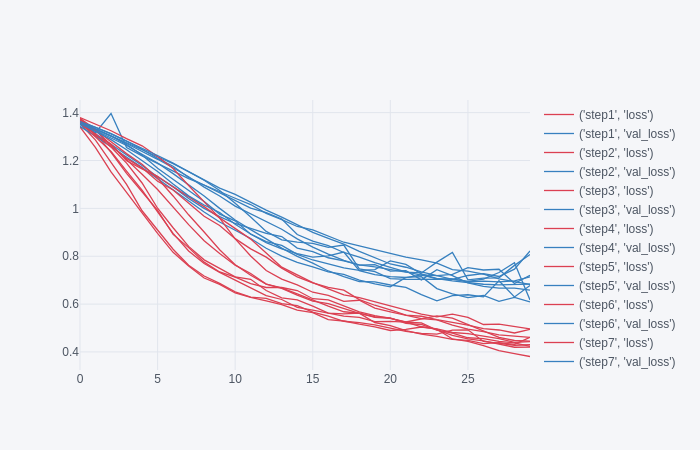
\includegraphics[width=0.75\textwidth]{imaxes/gn-3.png}
	\caption{Evolución modelo LSTM con normalización de batch e inicialización Glorot.}
	\label{gn-3}
\end{figure}

\begin{figure}[H]
	\centering
	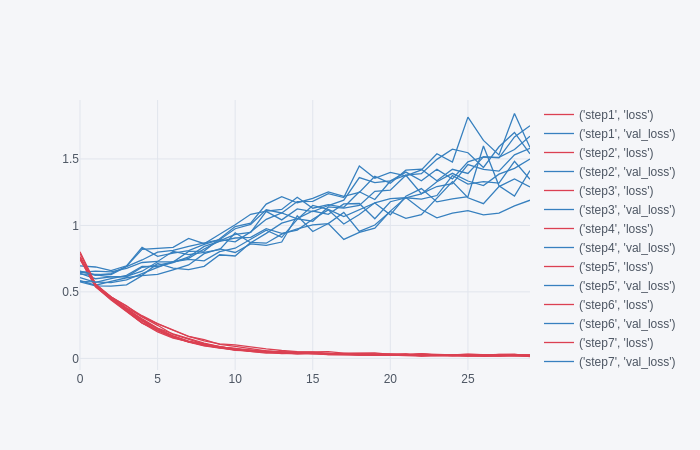
\includegraphics[width=0.75\textwidth]{imaxes/conv-3.png}
	\caption{Evolución modelo convolucional.}
	\label{conv-3}
\end{figure}

Si vemos las gráficas de evolución de los dos mejores modelos (figuras \ref{bn-3} y \ref{gn-3}) se observa una tendencia descendente que nos indica que podríamos obtener un mejor resultado afinando los parámetros o aumentando el número de iteraciones de entrenamiento. Por contra los modelos más complejos como el convolucional (fig. \ref{conv-3}) presentan sobre entrenamiento en fases tempranas del entrenamiento.

Los modelos complejos se comportan mejor en la clasificación con cambio de dominio.


\subsection{5 clases}

\begin{table}[H]
	\centering
	\begin{tabular}{|l|cccc|cccc|}
		\hline
		& \multicolumn{4}{c|}{TASS} & \multicolumn{4}{c|}{CINE} \\
		\cline{2-9}
		&    acc &     f1 &    mse &  recall & acc &     f1 &    mse &  recall \\
		\hline
		base          &  40.85 &  40.85 &  199.27 &   40.85 &  12.34 &  12.34 &  369.92 &   12.34 \\
		simpler       &  43.91 &  43.91 &  169.26 &   43.91 &  12.34 &  12.34 &  375.84 &   12.34 \\
		dropout   &  45.18 &  45.18 &  179.51 &   45.18  &   9.50 &   9.50 &  429.60 &    9.50\\
		batch norm    &  43.58 &  43.58 &  176.71 &   43.58 &   8.82 &   8.82 &  455.38 &    8.82\\
		glorot        &  45.51 &  45.51 &  201.60 &   45.51 &  11.76 &  11.76 &  382.44 &   11.76 \\
		glorot\_wo\_bn  &  43.05 &  43.05 &  176.31 &   43.05 &  13.24 &  13.24 &  357.64 &   13.24 \\
		double        &  41.85 &  41.85 &  142.38 &   41.85 &  21.80 &  \textbf{21.80} &  219.12 &   21.80\\
		conv          &  49.30 &  \textbf{49.30} &  214.77 &   49.30 &   9.14 &   9.14 &  443.42 &    9.14\\
		conv2d        &  43.11 &  43.11 &  182.97 &   43.11 &  11.26 &  11.26 &  400.44 &   11.26\\
		bidirectional &  45.51 &  45.51 &  182.37 &   45.51 &  12.00 &  12.00 &  396.64 &   12.00\\
		\hline
	\end{tabular}
	\caption{Resultados sobre el conjunto de test.}
	\label{test-dl-5-clases}
\end{table}

A pesar de que el mejor resultado en este experimento lo obtiene una red convolucional, vemos en la fig. \ref{conv-5} que durante su entrenamiento se ha producido un sobreentrenamiento.

Por otro lado los modelos Glorot con normalización de batch y sin ella presentan una tendencia a la baja como se ve en las figuras \ref{go-5} y \ref{gn-5} por lo que tenemos margen de mejora modificando hiperparámetros o ampliando el número de iteraciones hasta que se deje de apreciar una tendencia descendente en el entrenamiento.


\begin{figure}[H]
	\centering
	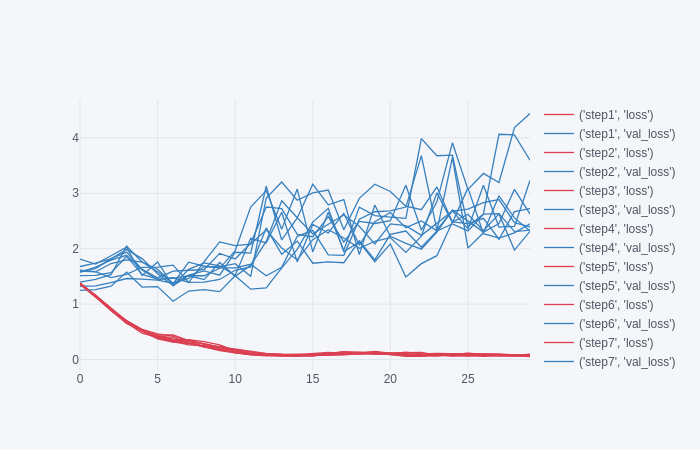
\includegraphics[width=0.75\textwidth]{imaxes/conv-5-clases.png}
	\caption{Evolución modelo convolucional.}
	\label{conv-5}
\end{figure}

\begin{figure}[H]
	\centering
	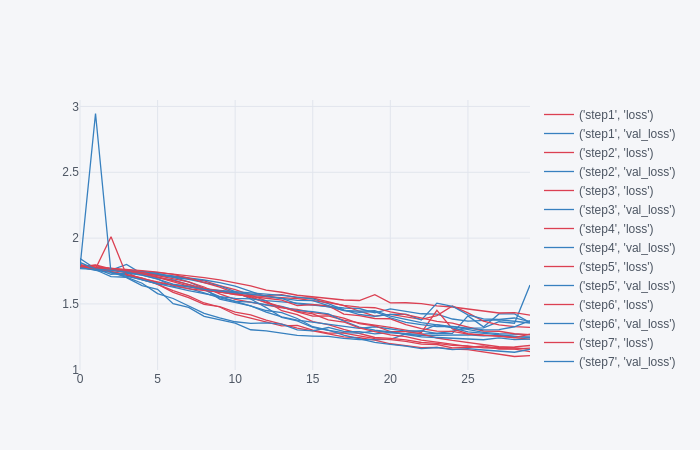
\includegraphics[width=0.75\textwidth]{imaxes/go.png}
	\caption{Evolución modelo LSTM con normalización de batch e inicialización Glorot.}
	\label{go-5}
\end{figure}

\begin{figure}[H]
	\centering
	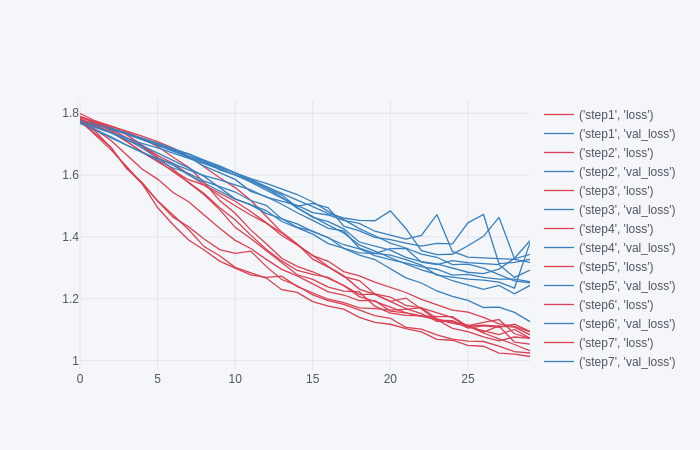
\includegraphics[width=0.75\textwidth]{imaxes/gnbn.png}
	\caption{Evolución modelo LSTM con normalización de batch.}
	\label{gn-5}
\end{figure}


\subsection{Conclusiones}

Tras analizar los resultados de las secciones anteriores podemos concluir que la complejidad del modelo no está directamente relacionada con su precisión ya que han sido los modelos más simples los que han obtenido mejor resultado. Destacando entre estos los modelos con inicialización Glorot, normalización del batch o una combinación entre ambos.

Las topologías complejas tienen tendencia a adaptarse muy rápido a los conjuntos de entrenamiento provocando un sobre entrenamiento. Esto puede ser debido a la simplicidad del conjunto de datos utilizado.

Podemos concluir que para la puesta en producción deberíamos utilizar los modelos de Deep Learning.

Además hemos demostrado que el corpus propuesto para los entrenamientos no nos garantiza los resultados finales, dado que desconocemos como van a ser los comentarios finales publicados en la aplicación. En estos experimentos hemos demostrado que si los documentos tienen mayor dimensionalidad que el corpus TASS se puede producir pérdida de información al cambiar de dominio y por lo tanto conseguir un peor rendimiento de los modelos.

Sería recomendable comenzar con una clasificación por umbrales, de forma que solo resulten clasificados automáticamente aquellos textos que tengan una probabilidad de pertenecer a una clase mayor a un tanto por ciento establecido entre la empresa y el cliente, además de ofrecer al usuario la posibilidad de clasificar su comentario, de esta forma dispondríamos de un corpus de comentarios con un valor establecido por humanos.

Cuando la aplicación cuente con un número de comentarios suficiente sería posible utilizarlos como corpus de entrenamiento.





 \chapter{Solución desarrollada}

\lettrine{E}{n} este capítulo mostraremos una serie de capturas de la solución desarrollada, centrándonos en la parte que se refiere a la resolución de los casos de uso expuestos en \ref{chap:cu}.

\section{Sección de comentarios}

\begin{figure}[H]
	\centering
	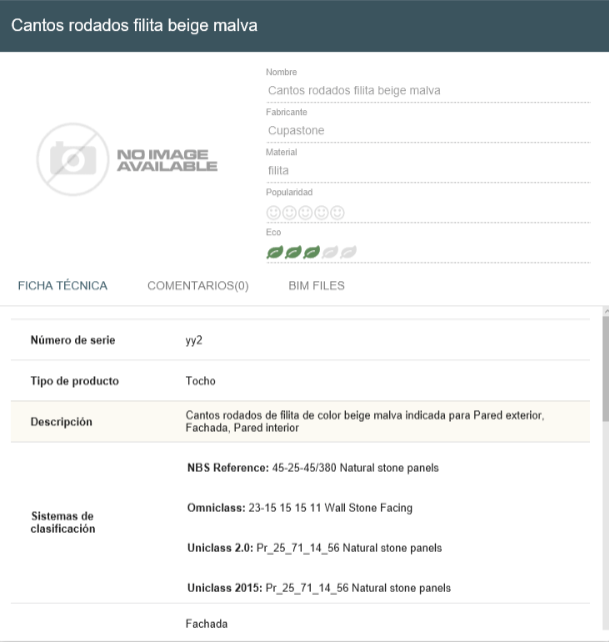
\includegraphics[width=0.5\textwidth]{imaxes/sectComment.png}
	\label{seccom}
	\caption{Sección de comentarios en la ficha de artículo.}
\end{figure}


\section{Publicación de comentarios}

\begin{figure}[H]
	\centering
	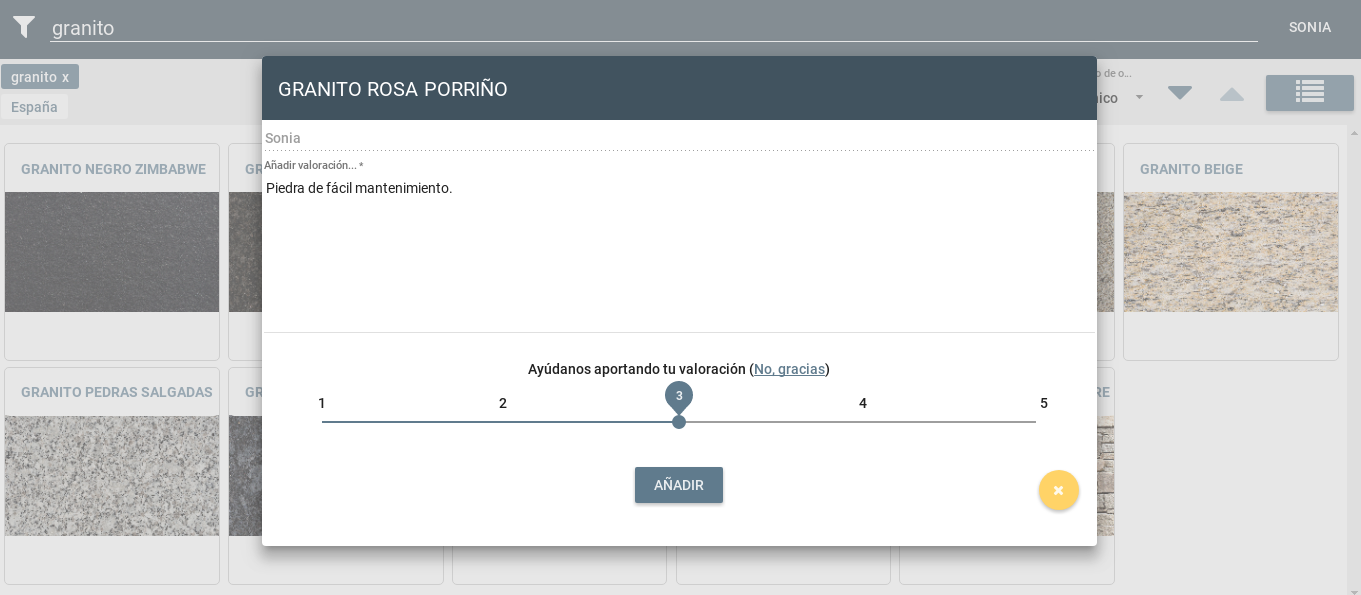
\includegraphics[width=0.75\textwidth]{imaxes/publicComment.png}
	\label{pubcom}
	\caption{Publicación de comentarios.}
\end{figure}

\section{Edición y eliminación de comentarios}

\begin{figure}[H]
	\centering
	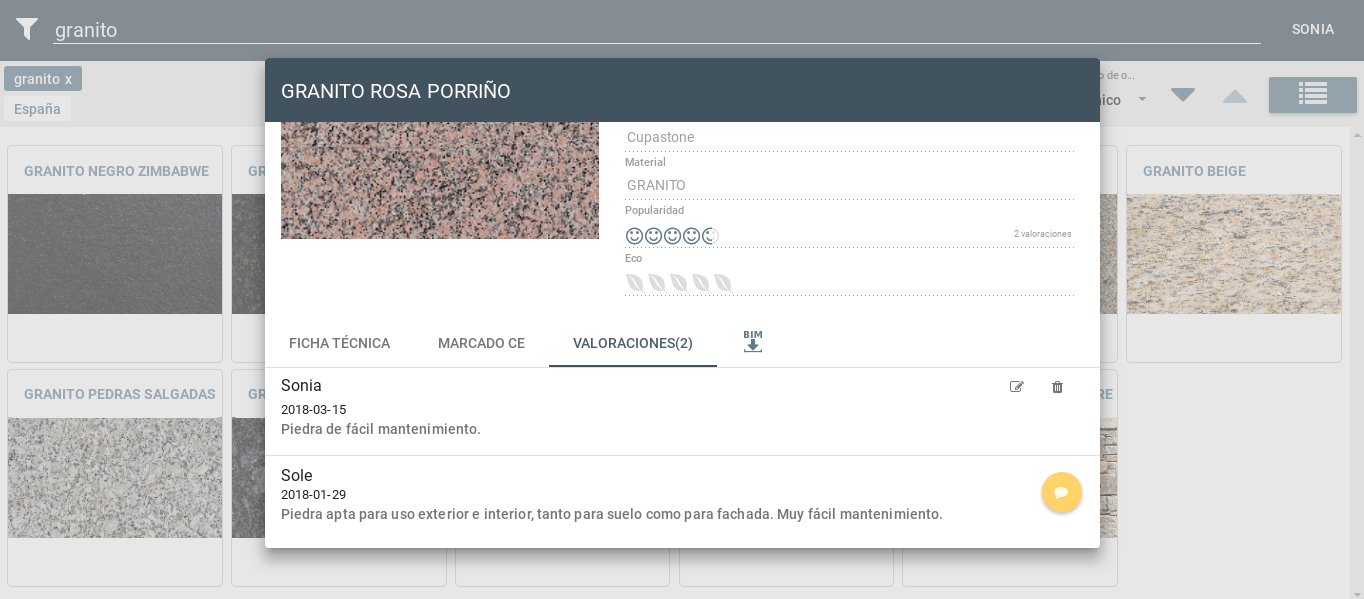
\includegraphics[width=0.75\textwidth]{imaxes/editComment.png}
	\label{edcom}
	\caption{Edición y eliminación de comentarios.}
\end{figure}

\paragraph{Trabajo futuro}

En el apartado de contenido extra se incluyen una serie de capturas que documentan una propuesta de rediseño y modernización de la interfaz.
%\include{contido/...}

 %%%%%%%%%%%%%%%%%%%%%%%%%%%%%%%%%%%%%%%%
 % Apéndices, glosarios e bibliografía  %
 %%%%%%%%%%%%%%%%%%%%%%%%%%%%%%%%%%%%%%%%

 \appendix
 \appendixpage
 \chapter{Material adicional}
\label{chap:adicional}

\section {Análisis de resultados}

\subsection{Línea base - 5 clases}\label{analisis_bl_5}

En la figura \ref{distTassCine} se aprecia una gran diferencia en la distribución de clases, mostrando en las polaridades del conjunto de entrenamiento una tendencia de agrupación en torno a los extremos, mientras que en el conjunto de test se agrupan en torno a la neutralidad. 

\begin{figure}[H]
	\centering
	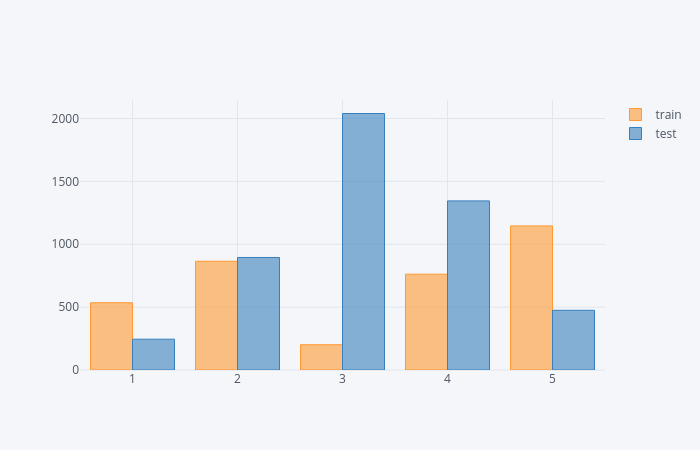
\includegraphics[width=1\textwidth]{imaxes/distCineTass.png}
	\caption{Distribución de polaridades en los conjuntos de entrenamiento y test.}
	\label{distTassCine}
\end{figure}

Este desbalanceo es una de las causas de los problemas de clasificación en distinto dominio, ya que el modelo tiende a clasificar los documentos con las polaridades que más destacan en el conjunto de entrenamiento, en este caso las clases con etiquetas 2 y 5, como se ve en la matriz de confusión representada en la figura \ref{conf5clases}.



\begin{figure}[H]
	\centering
	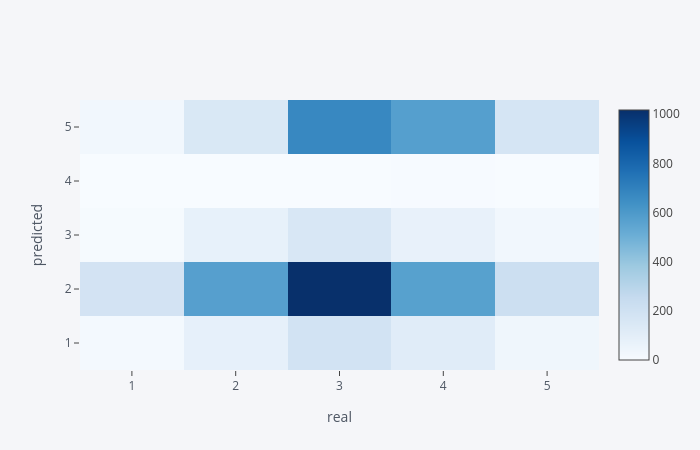
\includegraphics[width=1\textwidth]{imaxes/heatmap.png}
	\caption{Matriz de confusión de la clasificación en 5 clases.}
	\label{conf5clases}
\end{figure}


\section{Resultados GridSearch en Machine Learning}

\subsection{2 clases}

\begin{table}[H]
	\centering
	\begin{tabular}{|l|cccc|cccc|}
		\hline
		& \multicolumn{4}{c|}{CountVectorizer} & \multicolumn{4}{c|}{TF-IDF} \\
		\cline{2-9}
		&    acc &     f1 &    mse &  recall & acc &     f1 &    mse &  recall \\
		\hline
		lr      &  76.88 &  80.87 &  23.12 &   77.77 &  79.22 &  82.04 &  20.78 &   82.29 \\
		ls      &  76.60 &  80.52 &  23.40 &   77.85 &  80.99 &  \textbf{83.21} &  19.01 &   85.35 \\
		mb      &  79.93 &  \textbf{82.39} &  20.07 &   83.90 &  77.38 &  81.89 &  22.62 &   76.46 \\
		rf      &  73.55 &  77.10 &  26.45 &   77.44 &  70.92 &  74.85 &  29.08 &   75.12 \\
		\hline
	\end{tabular}
	\caption{Resultados en \% del mejor modelo obtenido en los k-folds}
	\label{result-cv-test}
\end{table}

\begin{table}[H]
	\centering
	\begin{tabular}{|l|cccc|cccc|}
		\hline
		& \multicolumn{4}{c|}{CountVectorizer} & \multicolumn{4}{c|}{TF-IDF} \\
		\cline{2-9}
		&    acc &     f1 &    mse &  recall & acc &     f1 &    mse &  recall \\
		\hline
		lr      &  63.44 &  \textbf{69.51} &  36.56 &   63.82 &  65.02 &  72.47 &  34.98 &   66.30 \\
		ls      &  62.55 &  65.74 &  37.45 &   65.66 &  64.56 &  73.09 &  35.44 &   64.97 \\
		mb      &  60.34 &  54.67 &  39.66 &   72.72 &  60.88 &  \textbf{73.29} &  39.12 &   60.41 \\
		rf      &  52.69 &  56.06 &  47.31 &   56.87 &  50.16 &  41.53 &  49.84 &   64.08 \\
		\hline
	\end{tabular}
	\caption{Resultados de la clasificación en el dominio de críticas de cine.}
	\label{result-cv-test-cine}
\end{table}

\subsection{3 clases}

\begin{table}[H]
	\centering
	\begin{tabular}{|l|cccc|cccc|}
		\hline
		& \multicolumn{4}{c|}{CountVectorizer} & \multicolumn{4}{c|}{TF-IDF} \\
		\cline{2-9}
		&    acc &     f1 &    mse &  recall & acc &     f1 &    mse &  recall \\
		\hline
		lr      &  67.86 &  67.86 &  105.59 &   67.86 &  74.32 &  74.32 &  80.37 &   74.32 \\
		ls      &  67.80 &  67.80 &  106.45 &   67.80 &  75.25 &  \textbf{75.25} &  76.65 &   75.25 \\
		mb      &  70.13 &  \textbf{70.13} &   96.74 &   70.13 &  71.86 &  71.86 &  90.22 &   71.86 \\
		rf      &  64.01 &  64.01 &  116.23 &   64.01 &  69.66 &  69.66 &  98.80 &   69.66 \\
		\hline
	\end{tabular}
	\caption{Resultados en \% del mejor modelo obtenido en los k-folds}
	\label{result-cv-test-3-clases}
\end{table}

\begin{table}[H]
	\centering
	\begin{tabular}{|l|cccc|cccc|}
		\hline
		& \multicolumn{4}{c|}{CountVectorizer} & \multicolumn{4}{c|}{TF-IDF} \\
		\cline{2-9}
		&    acc &     f1 &    mse &  recall & acc &     f1 &    mse &  recall \\
		\hline
		lr      &  39.74 &  \textbf{39.74} &  118.28 &   39.74 &  38.74 &  38.74 &  122.64 &   38.74\\
		ls      &  38.36 &  38.36 &  124.34 &   38.36 &  38.86 &  \textbf{38.86} &  122.16 &   38.86 \\
		mb      &  36.06 &  36.06 &  133.36 &   36.06 &  37.14 &  37.14 &  129.04 &   37.14 \\
		rf      &  34.94 &  34.94 &  119.24 &   34.94 &  34.42 &  34.42 &  139.92 &   34.42 \\
		\hline
	\end{tabular}
	\caption{Resultados de la clasificación en el dominio de críticas de cine.}
	\label{result-cv-test-3-clases-cine}
\end{table}

\subsection{5 clases}

\begin{table}[H]
	\centering
	\begin{tabular}{|l|cccc|cccc|}
		\hline
		& \multicolumn{4}{c|}{CountVectorizer} & \multicolumn{4}{c|}{TF-IDF} \\
		\cline{2-9}
		&    acc &     f1 &    mse &  recall & acc &     f1 &    mse &  recall \\
		\hline
		lr      &  41.05 &  41.05 &  268.06 &   41.05 &  45.58 &  45.58 &  222.82 &   45.58 \\
		ls      &  40.79 &  40.79 &  299.14 &   40.79 &  46.04 &  \textbf{46.04} &  214.90 &   46.04 \\
		mb      &  42.12 &  \textbf{42.12} &  257.29 &   42.12 &  42.38 &  42.38 &  285.56 &   42.38 \\
		rf      &  36.13 &  36.13 &  287.09 &   36.13 &  43.65 &  43.65 &  248.17 &   43.65 \\
		\hline
	\end{tabular}
	\caption{Resultados en \% del mejor modelo obtenido en los k-folds}
	\label{result-cv-test-5-clases}
\end{table}

\begin{table}[H]
	\centering
	\begin{tabular}{|l|cccc|cccc|}
		\hline
		& \multicolumn{4}{c|}{CountVectorizer} & \multicolumn{4}{c|}{TF-IDF} \\
		\cline{2-9}
		&    acc &     f1 &    mse &  recall & acc &     f1 &    mse &  recall \\
		\hline
		lr      &  14.08 &  14.08 &  373.52 &   14.08 &  13.54 &  13.54 &  360.28 &   13.54\\
		ls      &  12.44 &  12.44 &  384.74 &   12.44 &  12.70 &  12.70 &  376.00 &   12.70\\
		mb      &  18.52 &  18.52 &  267.64 &   18.52 &  11.56 &  11.56 &  390.06 &   11.56 \\
		rf      &  21.38 &  \textbf{21.38} &  257.68 &   21.38 &  15.26 &  \textbf{15.26} &  334.78 &   15.26 \\
		\hline
	\end{tabular}
	\caption{Resultados de la clasificación en el dominio de críticas de cine.}
	\label{result-cv-test-5-clases-cine}
\end{table}

\section{Trabajo futuro diseño web}

Con la intención de mejorar la UX/UI de la aplicación web, se plantea un rediseño enfocado a la minimalización y simplificación de la misma.

Se plantea el diseño entorno a 3 puntos:

\begin{description}
	\item [UX simple]: Un usuario debería saber que puede hacer en la aplicación de un vistazo. Una interfaz poco intuitiva puede suponer la frustración y por lo tanto pérdida de muchos usuarios.
	\item [Adaptarnos a la imagen de empresa]: Se deben seguir los estándares de diseño de la empresa cliente, véase: utilizar su logo, su paleta de colores, etc. Esto permitirá al cliente suavizar el impacto de la implantación de la herramienta en su ecosistema.
	\item [Enfocada en el producto]: Enfocar la interfaz al contenido importante, el producto.
\end{description}

\subsection{Página principal}

\begin{figure}[H]
	\centering
	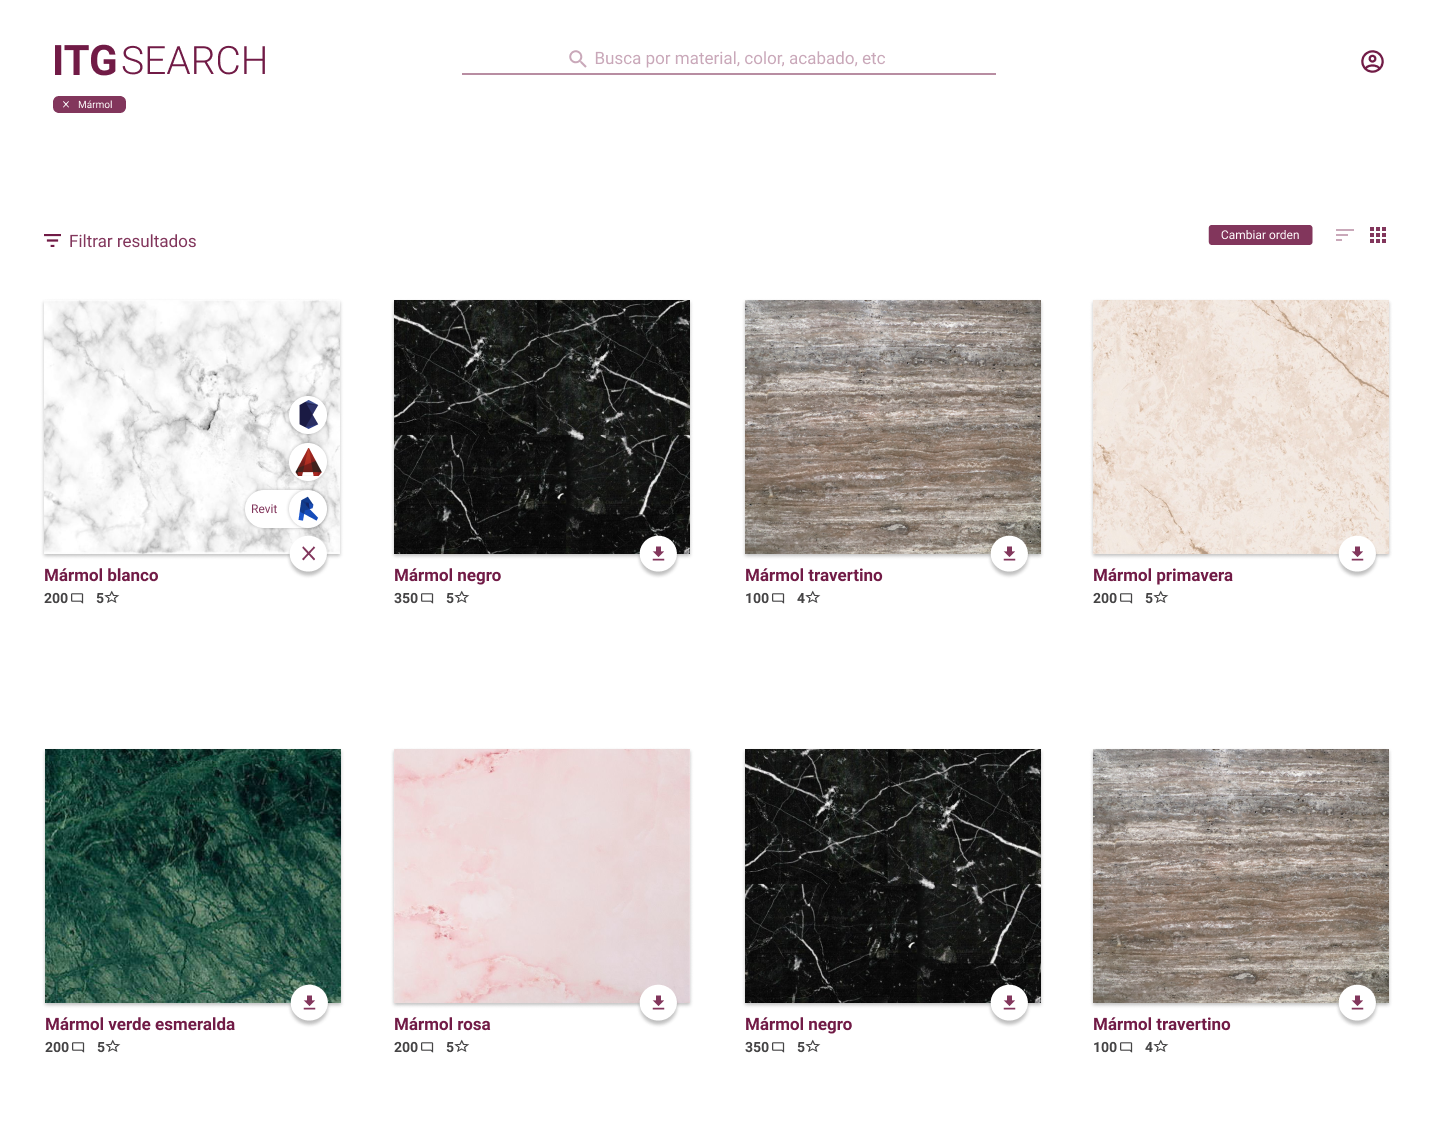
\includegraphics[width=1\textwidth]{imaxes/redHome.png}
	\caption{Página principal.}
	\label{redhome}
\end{figure}

Como vemos en la figura anterior hemos simplificado la interfaz y adoptado la paleta de colores de la empresa cliente.

A primera vista el usuario verá los artículos más destacados y toda la información relevante sobre los mimos, como número de comentarios, valoración y botón de descarga.

En este diseño asumimos el correcto funcionamiento del buscador, por lo que el usuario debería ser capaz de encontrar lo que desea entre los primeros 6 o 9 productos.

\subsection{Ficha de producto}

\begin{figure}[H]
	\centering
	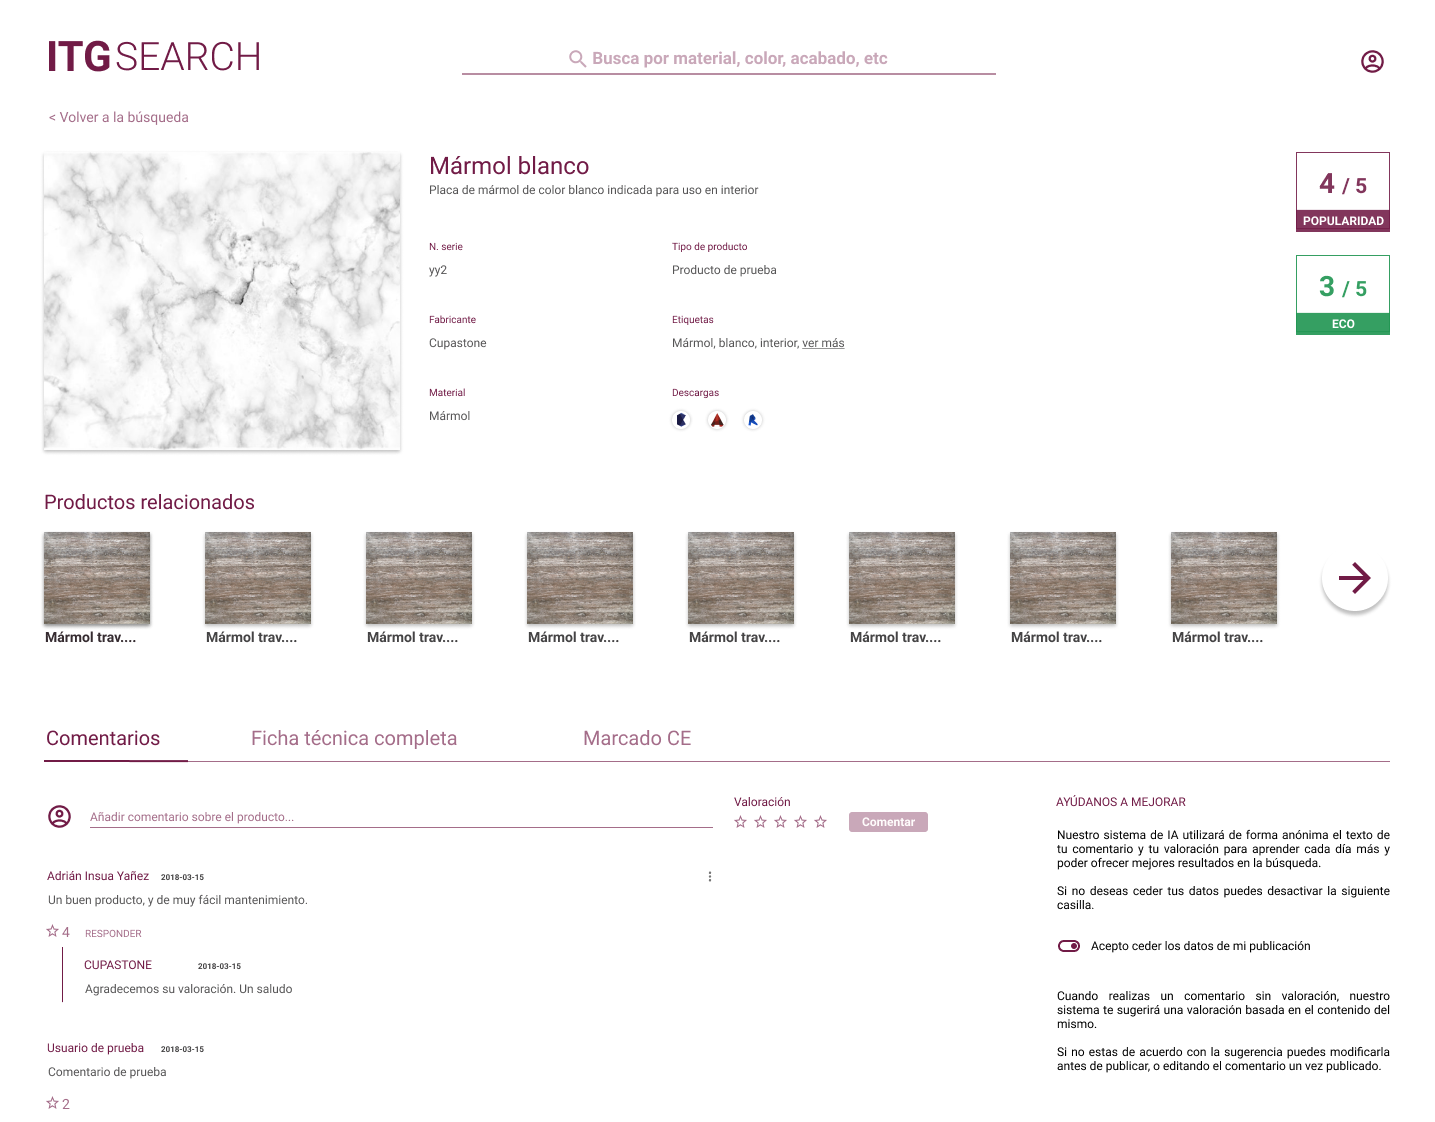
\includegraphics[width=1\textwidth]{imaxes/redProdDet.png}
	\caption{Ficha de producto.}
	\label{redProd}
\end{figure}

Para esta sección proponemos cambiar el modelo de ventana modal a una navegación completa, lo que nos permite introducir más información relevante sobre el artículo, sin que resulte molesto.

En esta ficha vemos además una sección de artículos relacionados, típica de las webs actuales, que se obtendrán a partir de las etiquetas del producto actual.

En la parte inferior se encuentra la sección de comentarios, y otras secciones secundarias. Hemos incluido el cuadro de inserción de comentarios y la nota sobre el uso de datos para mejorar el sistema de inteligencia artificial en la parte derecha de la sección de comentarios, evitando al usuario tener que dar pasos innecesarios.


%\include{anexos/...}

 \chapter*{\nomeglosarioacronimos}
\addcontentsline{toc}{chapter}{\nomeglosarioacronimos}
\label{chap:acronimos}
\thispagestyle{plain}
\fancyhead{}

%%%%%%%%%%%%%%%%%%%%%%%%%%%%%%%%%%%%%%%%%%%%%%%%%%%%%%%%%%%%%%%%%%%%%%%%%%%%%%%%
% Obxectivo: Lista de siglas, abreviaturas, acrónimos, etc. empregados         %
%            no documento, xunto cos seus respectivos significados.            %
%%%%%%%%%%%%%%%%%%%%%%%%%%%%%%%%%%%%%%%%%%%%%%%%%%%%%%%%%%%%%%%%%%%%%%%%%%%%%%%%

\begin{description}
\item [MNB] \emph{Multinomial Naive Bayes}
\item [LR] \emph {Logistic Regression}
\item [SVM] \emph {Support Vector Machines}
 \item [RF] \emph{Random Forest}.
\end{description}

%%%%%%%%%%%%%%%%%%%%%%%%%%%%%%%%%%%%%%%%%%%%%%%%%%%%%%%%%%%%%%%%%%%%%%%%%%%%%%%%

 \chapter*{\nomeglosariotermos}
\addcontentsline{toc}{chapter}{\nomeglosariotermos}
\label{chap:glosario-termos}

%%%%%%%%%%%%%%%%%%%%%%%%%%%%%%%%%%%%%%%%%%%%%%%%%%%%%%%%%%%%%%%%%%%%%%%%%%%%%%%%
% Obxectivo: Lista de termos empregados no documento,                          %
%            xunto cos seus respectivos significados.                          %
%%%%%%%%%%%%%%%%%%%%%%%%%%%%%%%%%%%%%%%%%%%%%%%%%%%%%%%%%%%%%%%%%%%%%%%%%%%%%%%%

\begin{description}
  
  \item [Corpus]
  Un corpus es un conjunto de documentos que se utilizarán como entrada para un sistema de análisis de sentimientos. Dichos documentos poseen una clasificación previa y generalmente realizada por humanos.
  
  \item[Lexicón de polaridad]
  
  Vocabulario que relaciona una palabra con una polaridad determinada, basada en la teoría de las emociones básicas del ser humano propuesta por Plutchik (\cite{Plutchick62},\cite{Plutchick80},\cite{Plutchick85})
  
  Para el trabajo se ha utilizado el diccionario término-emoción creado por Mohammad y Turney \cite{Lexicon} a través del servicio Mechanical Turk de Amazon, sobre el que se han realizado algunas correcciones de errores derivadas de la traducción automática de los términos mediante el servicio de traducción de Google.
  
  \item[Feature]
  
  Con este término nos referiremos a las características o propiedades de los textos que utilizaremos para predecir su polaridad mediante los distintos modelos de clasificación.
  
  \item[N-grama]
  
  Según la definición de Wikipedia\footnote{https://es.wikipedia.org/wiki/N-grama}: \textit{un n-grama es una subsecuencia de n elementos de una secuencia dada}. 
  Para el estudio del lenguaje los n-gramas son composiciones generalmente formadas por fonemas, sílabas, letras o palabras. 
  Los n-gramas se clasificarán según el valor de n:
  \begin{itemize}
  	\item unigrama: n-gramas de 1 solo elemento.
  	\item bigrama: n-grama de 2 elementos, también llamados digramas.
  	\item trigrama: n-grama de 3 elementos.
  \end{itemize}
  
  \item[Token]
  
  Cadena de caracteres que forman un componente léxico básico del sistema para la realización de la clasificación.
  
  Una sentencia está compuesta por una colección de tokens que corresponderán a las palabras que la forman.
  
  Frase: \textit{``La clasificación de textos en español"}.
  
  Tokens: [la, clasificación, de, textos, en, español]
  
  Si nos ceñimos al modelo de n-gramas un token sería considerado un unigrama.
  
  \item[Stopwords]
  
  Colección de palabras de uso común en un idioma, que dado que no aportan información relevante sobre los textos pueden ser eliminadas en un proceso previo de limpieza.
  
  Comúnmente esta colección está formada por preposiciones, pronombres, verbos comunes, signos de puntuación, y otras palabras dependientes del dominio del problema.
  
  \item[Preprocesamiento]
  
  Proceso de tratamiento previo de los datos que pretende mejorar la calidad de los mismos. Dado que se trata de un dominio no profesional es común encontrar faltas de ortografía cometidas por los usuarios, caracteres especiales del dominio (hashtags o menciones de twitter, emoticonos, etc.) que no aportan información válida para la tarea, y necesitaremos deshacernos de ellos antes de utilizar los textos.
\end{description}

\nocite{*}
 \bibliographystyle{IEEEtran}
 \bibliography{\bibconfig,bibliografia/bibliografia}
 \cleardoublepage
 
\end{document}

%%%%%%%%%%%%%%%%%%%%%%%%%%%%%%%%%%%%%%%%%%%%%%%%%%%%%%%%%%%%%%%%%%%%%%%%%%%%%%%%
